\documentclass[twoside]{book}

% Packages required by doxygen
\usepackage{fixltx2e}
\usepackage{calc}
\usepackage{doxygen}
\usepackage[export]{adjustbox} % also loads graphicx
\usepackage{graphicx}
\usepackage[utf8]{inputenc}
\usepackage{makeidx}
\usepackage{multicol}
\usepackage{multirow}
\PassOptionsToPackage{warn}{textcomp}
\usepackage{textcomp}
\usepackage[nointegrals]{wasysym}
\usepackage[table]{xcolor}

% NLS support packages
\usepackage[french]{babel}

% Font selection
\usepackage[T1]{fontenc}
\usepackage[scaled=.90]{helvet}
\usepackage{courier}
\usepackage{amssymb}
\usepackage{sectsty}
\renewcommand{\familydefault}{\sfdefault}
\allsectionsfont{%
  \fontseries{bc}\selectfont%
  \color{darkgray}%
}
\renewcommand{\DoxyLabelFont}{%
  \fontseries{bc}\selectfont%
  \color{darkgray}%
}
\newcommand{\+}{\discretionary{\mbox{\scriptsize$\hookleftarrow$}}{}{}}

% Page & text layout
\usepackage{geometry}
\geometry{%
  a4paper,%
  top=2.5cm,%
  bottom=2.5cm,%
  left=2.5cm,%
  right=2.5cm%
}
\tolerance=750
\hfuzz=15pt
\hbadness=750
\setlength{\emergencystretch}{15pt}
\setlength{\parindent}{0cm}
\setlength{\parskip}{3ex plus 2ex minus 2ex}
\makeatletter
\renewcommand{\paragraph}{%
  \@startsection{paragraph}{4}{0ex}{-1.0ex}{1.0ex}{%
    \normalfont\normalsize\bfseries\SS@parafont%
  }%
}
\renewcommand{\subparagraph}{%
  \@startsection{subparagraph}{5}{0ex}{-1.0ex}{1.0ex}{%
    \normalfont\normalsize\bfseries\SS@subparafont%
  }%
}
\makeatother

% Headers & footers
\usepackage{fancyhdr}
\pagestyle{fancyplain}
\fancyhead[LE]{\fancyplain{}{\bfseries\thepage}}
\fancyhead[CE]{\fancyplain{}{}}
\fancyhead[RE]{\fancyplain{}{\bfseries\leftmark}}
\fancyhead[LO]{\fancyplain{}{\bfseries\rightmark}}
\fancyhead[CO]{\fancyplain{}{}}
\fancyhead[RO]{\fancyplain{}{\bfseries\thepage}}
\fancyfoot[LE]{\fancyplain{}{}}
\fancyfoot[CE]{\fancyplain{}{}}
\fancyfoot[RE]{\fancyplain{}{\bfseries\scriptsize Généré par Doxygen }}
\fancyfoot[LO]{\fancyplain{}{\bfseries\scriptsize Généré par Doxygen }}
\fancyfoot[CO]{\fancyplain{}{}}
\fancyfoot[RO]{\fancyplain{}{}}
\renewcommand{\footrulewidth}{0.4pt}
\renewcommand{\chaptermark}[1]{%
  \markboth{#1}{}%
}
\renewcommand{\sectionmark}[1]{%
  \markright{\thesection\ #1}%
}

% Indices & bibliography
\usepackage{natbib}
\usepackage[titles]{tocloft}
\setcounter{tocdepth}{3}
\setcounter{secnumdepth}{5}
\makeindex

% Hyperlinks (required, but should be loaded last)
\usepackage{ifpdf}
\ifpdf
  \usepackage[pdftex,pagebackref=true]{hyperref}
\else
  \usepackage[ps2pdf,pagebackref=true]{hyperref}
\fi
\hypersetup{%
  colorlinks=true,%
  linkcolor=blue,%
  citecolor=blue,%
  unicode%
}

% Custom commands
\newcommand{\clearemptydoublepage}{%
  \newpage{\pagestyle{empty}\cleardoublepage}%
}

\usepackage{caption}
\captionsetup{labelsep=space,justification=centering,font={bf},singlelinecheck=off,skip=4pt,position=top}

%===== C O N T E N T S =====

\begin{document}

% Titlepage & ToC
\hypersetup{pageanchor=false,
             bookmarksnumbered=true,
             pdfencoding=unicode
            }
\pagenumbering{alph}
\begin{titlepage}
\vspace*{7cm}
\begin{center}%
{\Large Image Tagger }\\
\vspace*{1cm}
{\large Généré par Doxygen 1.8.13}\\
\end{center}
\end{titlepage}
\clearemptydoublepage
\pagenumbering{roman}
\tableofcontents
\clearemptydoublepage
\pagenumbering{arabic}
\hypersetup{pageanchor=true}

%--- Begin generated contents ---
\chapter{Index hiérarchique}
\section{Hiérarchie des classes}
Cette liste d\textquotesingle{}héritage est classée approximativement par ordre alphabétique \+:\begin{DoxyCompactList}
\item \contentsline{section}{Collection$<$ T $>$}{\pageref{class_collection}}{}
\begin{DoxyCompactList}
\item \contentsline{section}{Collection\+Pool$<$ T $>$}{\pageref{class_collection_pool}}{}
\item \contentsline{section}{Filtered\+Collection$<$ T $>$}{\pageref{class_filtered_collection}}{}
\end{DoxyCompactList}
\item \contentsline{section}{Collection\+Iterator$<$ T $>$}{\pageref{class_collection_iterator}}{}
\item \contentsline{section}{Image$<$ img\+\_\+t $>$}{\pageref{class_image}}{}
\item \contentsline{section}{Iterator\+Base$<$ T $>$}{\pageref{class_iterator_base}}{}
\begin{DoxyCompactList}
\item \contentsline{section}{Filtered\+Iterator$<$ T $>$}{\pageref{class_filtered_iterator}}{}
\item \contentsline{section}{Pool\+Iterator$<$ T $>$}{\pageref{class_pool_iterator}}{}
\end{DoxyCompactList}
\end{DoxyCompactList}

\chapter{Index des classes}
\section{Liste des classes}
Liste des classes, structures, unions et interfaces avec une brève description \+:\begin{DoxyCompactList}
\item\contentsline{section}{\hyperlink{class_collection}{Collection$<$ T $>$} }{\pageref{class_collection}}{}
\item\contentsline{section}{\hyperlink{class_collection_iterator}{Collection\+Iterator$<$ T $>$} }{\pageref{class_collection_iterator}}{}
\item\contentsline{section}{\hyperlink{class_collection_pool}{Collection\+Pool$<$ T $>$} }{\pageref{class_collection_pool}}{}
\item\contentsline{section}{\hyperlink{structfile__filter}{file\+\_\+filter} }{\pageref{structfile__filter}}{}
\item\contentsline{section}{\hyperlink{class_filtered_collection}{Filtered\+Collection$<$ T $>$} }{\pageref{class_filtered_collection}}{}
\item\contentsline{section}{\hyperlink{class_filtered_iterator}{Filtered\+Iterator$<$ T $>$} }{\pageref{class_filtered_iterator}}{}
\item\contentsline{section}{\hyperlink{class_image}{Image$<$ img\+\_\+t $>$} }{\pageref{class_image}}{}
\item\contentsline{section}{\hyperlink{class_iterator_base}{Iterator\+Base$<$ T $>$} }{\pageref{class_iterator_base}}{}
\item\contentsline{section}{\hyperlink{class_pool_iterator}{Pool\+Iterator$<$ T $>$} }{\pageref{class_pool_iterator}}{}
\end{DoxyCompactList}

\chapter{Index des fichiers}
\section{Liste des fichiers}
Liste de tous les fichiers avec une brève description \+:\begin{DoxyCompactList}
\item\contentsline{section}{src/\hyperlink{_collection_8hpp}{Collection.\+hpp} }{\pageref{_collection_8hpp}}{}
\item\contentsline{section}{src/\hyperlink{_collection_iterator_8hpp}{Collection\+Iterator.\+hpp} }{\pageref{_collection_iterator_8hpp}}{}
\item\contentsline{section}{src/\hyperlink{_collection_pool_8hpp}{Collection\+Pool.\+hpp} }{\pageref{_collection_pool_8hpp}}{}
\item\contentsline{section}{src/\hyperlink{_file_dialog_8hpp}{File\+Dialog.\+hpp} }{\pageref{_file_dialog_8hpp}}{}
\item\contentsline{section}{src/\hyperlink{_file_dialog_linux_8cpp}{File\+Dialog\+Linux.\+cpp} }{\pageref{_file_dialog_linux_8cpp}}{}
\item\contentsline{section}{src/\hyperlink{_file_dialog_windows_8cpp}{File\+Dialog\+Windows.\+cpp} }{\pageref{_file_dialog_windows_8cpp}}{}
\item\contentsline{section}{src/\hyperlink{_filtered_collection_8hpp}{Filtered\+Collection.\+hpp} }{\pageref{_filtered_collection_8hpp}}{}
\item\contentsline{section}{src/\hyperlink{_image_8hpp}{Image.\+hpp} }{\pageref{_image_8hpp}}{}
\item\contentsline{section}{src/\hyperlink{main_8cpp}{main.\+cpp} }{\pageref{main_8cpp}}{}
\item\contentsline{section}{src/\hyperlink{system__target_8hpp}{system\+\_\+target.\+hpp} }{\pageref{system__target_8hpp}}{}
\item\contentsline{section}{src/\hyperlink{_tag_list_8hpp}{Tag\+List.\+hpp} }{\pageref{_tag_list_8hpp}}{}
\item\contentsline{section}{src/\hyperlink{_window_8hpp}{Window.\+hpp} }{\pageref{_window_8hpp}}{}
\end{DoxyCompactList}

\chapter{Documentation des classes}
\hypertarget{class_collection}{}\section{Référence du modèle de la classe Collection$<$ T $>$}
\label{class_collection}\index{Collection$<$ T $>$@{Collection$<$ T $>$}}


{\ttfamily \#include $<$Collection.\+hpp$>$}



Graphe d\textquotesingle{}héritage de Collection$<$ T $>$\+:\nopagebreak
\begin{figure}[H]
\begin{center}
\leavevmode
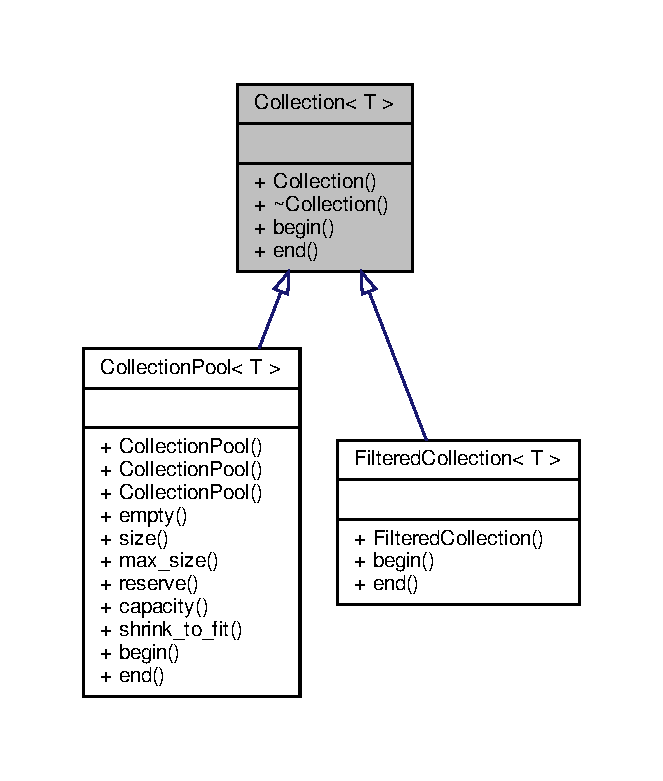
\includegraphics[width=318pt]{class_collection__inherit__graph}
\end{center}
\end{figure}


Graphe de collaboration de Collection$<$ T $>$\+:\nopagebreak
\begin{figure}[H]
\begin{center}
\leavevmode
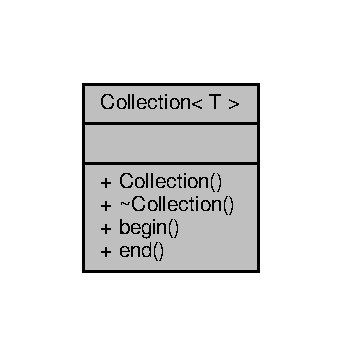
\includegraphics[width=164pt]{class_collection__coll__graph}
\end{center}
\end{figure}
\subsection*{Types publics}
\begin{DoxyCompactItemize}
\item 
using \hyperlink{class_collection_a30ecb2b5696f341f4b751019679c41e0}{value\+\_\+type} = T
\item 
using \hyperlink{class_collection_ac7974b0b552f0a94065aadc48ae53397}{allocator\+\_\+type} = std\+::allocator$<$ T $>$
\item 
using \hyperlink{class_collection_abbc291771b11c48cd2f297a0d9fe0449}{reference} = T \&
\item 
using \hyperlink{class_collection_abb8c0f6de5e322aa531837aab7358b89}{const\+\_\+reference} = const T \&
\item 
using \hyperlink{class_collection_a9a5b5d9b389c113364d527900c745efb}{pointer} = T $\ast$
\item 
using \hyperlink{class_collection_a79ea96d1fa145e340e907547d0053b81}{const\+\_\+pointer} = const T $\ast$
\item 
using \hyperlink{class_collection_a317dca4fdf1eb2e47643bb60c620f802}{iterator} = \hyperlink{class_collection_iterator}{Collection\+Iterator}$<$ T $>$
\item 
using \hyperlink{class_collection_ac3805407b2dc537e71db7af070b8d8a6}{reverse\+\_\+iterator} = std\+::reverse\+\_\+iterator$<$ \hyperlink{class_collection_a317dca4fdf1eb2e47643bb60c620f802}{iterator} $>$
\item 
using \hyperlink{class_collection_a60b36ef7aba0a88dff0e98fc2adb98a8}{difference\+\_\+type} = std\+::ptrdiff\+\_\+t
\item 
using \hyperlink{class_collection_a3f8b024f587aa20be530866da30948c4}{size\+\_\+type} = size\+\_\+t
\end{DoxyCompactItemize}
\subsection*{Fonctions membres publiques}
\begin{DoxyCompactItemize}
\item 
\hyperlink{class_collection_af6be61fb9648c2ac1ef7c8456b49a441}{Collection} ()=default
\item 
virtual \hyperlink{class_collection_ae9e3ec131717723e10152cb7ec3b0379}{$\sim$\+Collection} ()=default
\item 
virtual \hyperlink{class_collection_a317dca4fdf1eb2e47643bb60c620f802}{iterator} \hyperlink{class_collection_a4abc73f8e31a499a22b25d42b7a4fe8c}{begin} ()=0
\item 
virtual \hyperlink{class_collection_a317dca4fdf1eb2e47643bb60c620f802}{iterator} \hyperlink{class_collection_ab5b98f651d0f49cde1be067c69c52e89}{end} ()=0
\end{DoxyCompactItemize}


\subsection{Documentation des définitions de type membres}
\mbox{\Hypertarget{class_collection_ac7974b0b552f0a94065aadc48ae53397}\label{class_collection_ac7974b0b552f0a94065aadc48ae53397}} 
\index{Collection@{Collection}!allocator\+\_\+type@{allocator\+\_\+type}}
\index{allocator\+\_\+type@{allocator\+\_\+type}!Collection@{Collection}}
\subsubsection{\texorpdfstring{allocator\+\_\+type}{allocator\_type}}
{\footnotesize\ttfamily template$<$typename T$>$ \\
using \hyperlink{class_collection}{Collection}$<$ T $>$\+::\hyperlink{class_collection_ac7974b0b552f0a94065aadc48ae53397}{allocator\+\_\+type} =  std\+::allocator$<$T$>$}

\mbox{\Hypertarget{class_collection_a79ea96d1fa145e340e907547d0053b81}\label{class_collection_a79ea96d1fa145e340e907547d0053b81}} 
\index{Collection@{Collection}!const\+\_\+pointer@{const\+\_\+pointer}}
\index{const\+\_\+pointer@{const\+\_\+pointer}!Collection@{Collection}}
\subsubsection{\texorpdfstring{const\+\_\+pointer}{const\_pointer}}
{\footnotesize\ttfamily template$<$typename T$>$ \\
using \hyperlink{class_collection}{Collection}$<$ T $>$\+::\hyperlink{class_collection_a79ea96d1fa145e340e907547d0053b81}{const\+\_\+pointer} =  const T$\ast$}

\mbox{\Hypertarget{class_collection_abb8c0f6de5e322aa531837aab7358b89}\label{class_collection_abb8c0f6de5e322aa531837aab7358b89}} 
\index{Collection@{Collection}!const\+\_\+reference@{const\+\_\+reference}}
\index{const\+\_\+reference@{const\+\_\+reference}!Collection@{Collection}}
\subsubsection{\texorpdfstring{const\+\_\+reference}{const\_reference}}
{\footnotesize\ttfamily template$<$typename T$>$ \\
using \hyperlink{class_collection}{Collection}$<$ T $>$\+::\hyperlink{class_collection_abb8c0f6de5e322aa531837aab7358b89}{const\+\_\+reference} =  const T\&}

\mbox{\Hypertarget{class_collection_a60b36ef7aba0a88dff0e98fc2adb98a8}\label{class_collection_a60b36ef7aba0a88dff0e98fc2adb98a8}} 
\index{Collection@{Collection}!difference\+\_\+type@{difference\+\_\+type}}
\index{difference\+\_\+type@{difference\+\_\+type}!Collection@{Collection}}
\subsubsection{\texorpdfstring{difference\+\_\+type}{difference\_type}}
{\footnotesize\ttfamily template$<$typename T$>$ \\
using \hyperlink{class_collection}{Collection}$<$ T $>$\+::\hyperlink{class_collection_a60b36ef7aba0a88dff0e98fc2adb98a8}{difference\+\_\+type} =  std\+::ptrdiff\+\_\+t}

\mbox{\Hypertarget{class_collection_a317dca4fdf1eb2e47643bb60c620f802}\label{class_collection_a317dca4fdf1eb2e47643bb60c620f802}} 
\index{Collection@{Collection}!iterator@{iterator}}
\index{iterator@{iterator}!Collection@{Collection}}
\subsubsection{\texorpdfstring{iterator}{iterator}}
{\footnotesize\ttfamily template$<$typename T$>$ \\
using \hyperlink{class_collection}{Collection}$<$ T $>$\+::\hyperlink{class_collection_a317dca4fdf1eb2e47643bb60c620f802}{iterator} =  \hyperlink{class_collection_iterator}{Collection\+Iterator}$<$T$>$}

\mbox{\Hypertarget{class_collection_a9a5b5d9b389c113364d527900c745efb}\label{class_collection_a9a5b5d9b389c113364d527900c745efb}} 
\index{Collection@{Collection}!pointer@{pointer}}
\index{pointer@{pointer}!Collection@{Collection}}
\subsubsection{\texorpdfstring{pointer}{pointer}}
{\footnotesize\ttfamily template$<$typename T$>$ \\
using \hyperlink{class_collection}{Collection}$<$ T $>$\+::\hyperlink{class_collection_a9a5b5d9b389c113364d527900c745efb}{pointer} =  T$\ast$}

\mbox{\Hypertarget{class_collection_abbc291771b11c48cd2f297a0d9fe0449}\label{class_collection_abbc291771b11c48cd2f297a0d9fe0449}} 
\index{Collection@{Collection}!reference@{reference}}
\index{reference@{reference}!Collection@{Collection}}
\subsubsection{\texorpdfstring{reference}{reference}}
{\footnotesize\ttfamily template$<$typename T$>$ \\
using \hyperlink{class_collection}{Collection}$<$ T $>$\+::\hyperlink{class_collection_abbc291771b11c48cd2f297a0d9fe0449}{reference} =  T\&}

\mbox{\Hypertarget{class_collection_ac3805407b2dc537e71db7af070b8d8a6}\label{class_collection_ac3805407b2dc537e71db7af070b8d8a6}} 
\index{Collection@{Collection}!reverse\+\_\+iterator@{reverse\+\_\+iterator}}
\index{reverse\+\_\+iterator@{reverse\+\_\+iterator}!Collection@{Collection}}
\subsubsection{\texorpdfstring{reverse\+\_\+iterator}{reverse\_iterator}}
{\footnotesize\ttfamily template$<$typename T$>$ \\
using \hyperlink{class_collection}{Collection}$<$ T $>$\+::\hyperlink{class_collection_ac3805407b2dc537e71db7af070b8d8a6}{reverse\+\_\+iterator} =  std\+::reverse\+\_\+iterator$<$\hyperlink{class_collection_a317dca4fdf1eb2e47643bb60c620f802}{iterator}$>$}

\mbox{\Hypertarget{class_collection_a3f8b024f587aa20be530866da30948c4}\label{class_collection_a3f8b024f587aa20be530866da30948c4}} 
\index{Collection@{Collection}!size\+\_\+type@{size\+\_\+type}}
\index{size\+\_\+type@{size\+\_\+type}!Collection@{Collection}}
\subsubsection{\texorpdfstring{size\+\_\+type}{size\_type}}
{\footnotesize\ttfamily template$<$typename T$>$ \\
using \hyperlink{class_collection}{Collection}$<$ T $>$\+::\hyperlink{class_collection_a3f8b024f587aa20be530866da30948c4}{size\+\_\+type} =  size\+\_\+t}

\mbox{\Hypertarget{class_collection_a30ecb2b5696f341f4b751019679c41e0}\label{class_collection_a30ecb2b5696f341f4b751019679c41e0}} 
\index{Collection@{Collection}!value\+\_\+type@{value\+\_\+type}}
\index{value\+\_\+type@{value\+\_\+type}!Collection@{Collection}}
\subsubsection{\texorpdfstring{value\+\_\+type}{value\_type}}
{\footnotesize\ttfamily template$<$typename T$>$ \\
using \hyperlink{class_collection}{Collection}$<$ T $>$\+::\hyperlink{class_collection_a30ecb2b5696f341f4b751019679c41e0}{value\+\_\+type} =  T}



\subsection{Documentation des constructeurs et destructeur}
\mbox{\Hypertarget{class_collection_af6be61fb9648c2ac1ef7c8456b49a441}\label{class_collection_af6be61fb9648c2ac1ef7c8456b49a441}} 
\index{Collection@{Collection}!Collection@{Collection}}
\index{Collection@{Collection}!Collection@{Collection}}
\subsubsection{\texorpdfstring{Collection()}{Collection()}}
{\footnotesize\ttfamily template$<$typename T$>$ \\
\hyperlink{class_collection}{Collection}$<$ T $>$\+::\hyperlink{class_collection}{Collection} (\begin{DoxyParamCaption}{ }\end{DoxyParamCaption})\hspace{0.3cm}{\ttfamily [default]}}

\mbox{\Hypertarget{class_collection_ae9e3ec131717723e10152cb7ec3b0379}\label{class_collection_ae9e3ec131717723e10152cb7ec3b0379}} 
\index{Collection@{Collection}!````~Collection@{$\sim$\+Collection}}
\index{````~Collection@{$\sim$\+Collection}!Collection@{Collection}}
\subsubsection{\texorpdfstring{$\sim$\+Collection()}{~Collection()}}
{\footnotesize\ttfamily template$<$typename T$>$ \\
virtual \hyperlink{class_collection}{Collection}$<$ T $>$\+::$\sim$\hyperlink{class_collection}{Collection} (\begin{DoxyParamCaption}{ }\end{DoxyParamCaption})\hspace{0.3cm}{\ttfamily [virtual]}, {\ttfamily [default]}}



\subsection{Documentation des fonctions membres}
\mbox{\Hypertarget{class_collection_a4abc73f8e31a499a22b25d42b7a4fe8c}\label{class_collection_a4abc73f8e31a499a22b25d42b7a4fe8c}} 
\index{Collection@{Collection}!begin@{begin}}
\index{begin@{begin}!Collection@{Collection}}
\subsubsection{\texorpdfstring{begin()}{begin()}}
{\footnotesize\ttfamily template$<$typename T$>$ \\
virtual \hyperlink{class_collection_a317dca4fdf1eb2e47643bb60c620f802}{iterator} \hyperlink{class_collection}{Collection}$<$ T $>$\+::begin (\begin{DoxyParamCaption}{ }\end{DoxyParamCaption})\hspace{0.3cm}{\ttfamily [pure virtual]}}



Implémenté dans \hyperlink{class_collection_pool_ae13d478a26554da9211db064285c7b0b}{Collection\+Pool$<$ T $>$}, et \hyperlink{class_filtered_collection_a114f2b1557201e523a264d549926ab0a}{Filtered\+Collection$<$ T $>$}.

\mbox{\Hypertarget{class_collection_ab5b98f651d0f49cde1be067c69c52e89}\label{class_collection_ab5b98f651d0f49cde1be067c69c52e89}} 
\index{Collection@{Collection}!end@{end}}
\index{end@{end}!Collection@{Collection}}
\subsubsection{\texorpdfstring{end()}{end()}}
{\footnotesize\ttfamily template$<$typename T$>$ \\
virtual \hyperlink{class_collection_a317dca4fdf1eb2e47643bb60c620f802}{iterator} \hyperlink{class_collection}{Collection}$<$ T $>$\+::end (\begin{DoxyParamCaption}{ }\end{DoxyParamCaption})\hspace{0.3cm}{\ttfamily [pure virtual]}}



Implémenté dans \hyperlink{class_collection_pool_a870a85422595d6533688704ebe43b520}{Collection\+Pool$<$ T $>$}, et \hyperlink{class_filtered_collection_ae310c937df5035ef07f7d4de65fca18b}{Filtered\+Collection$<$ T $>$}.



La documentation de cette classe a été générée à partir du fichier suivant \+:\begin{DoxyCompactItemize}
\item 
src/\hyperlink{_collection_8hpp}{Collection.\+hpp}\end{DoxyCompactItemize}

\hypertarget{class_collection_iterator}{}\section{Référence du modèle de la classe Collection\+Iterator$<$ T $>$}
\label{class_collection_iterator}\index{Collection\+Iterator$<$ T $>$@{Collection\+Iterator$<$ T $>$}}


{\ttfamily \#include $<$Collection\+Iterator.\+hpp$>$}



Graphe de collaboration de Collection\+Iterator$<$ T $>$\+:\nopagebreak
\begin{figure}[H]
\begin{center}
\leavevmode
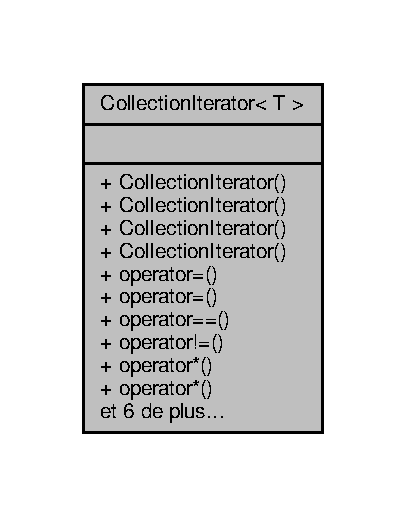
\includegraphics[width=195pt]{class_collection_iterator__coll__graph}
\end{center}
\end{figure}
\subsection*{Types publics}
\begin{DoxyCompactItemize}
\item 
using \hyperlink{class_collection_iterator_a0f4af23418960a0fe3889b5381d6a79c}{iterator\+\_\+category} = std\+::bidirectional\+\_\+iterator\+\_\+tag
\item 
using \hyperlink{class_collection_iterator_a8513f3c29655e48f34f8b6a11b96a71b}{value\+\_\+type} = T
\item 
using \hyperlink{class_collection_iterator_a9bff5744ce1cfc8f704fa52557699594}{const\+\_\+pointer} = const T $\ast$
\item 
using \hyperlink{class_collection_iterator_aff846a9c86022d66a7eb10e3623a0ba0}{pointer} = T $\ast$
\item 
using \hyperlink{class_collection_iterator_ab0f0742da5375882a74038d82de41aca}{const\+\_\+reference} = const T \&
\item 
using \hyperlink{class_collection_iterator_aac15417aa7a67fdfb86b8bad1b4d5ddf}{reference} = T \&
\item 
using \hyperlink{class_collection_iterator_a4dca8639d1f342073ccf8bcd4d27e3bf}{difference\+\_\+type} = std\+::ptrdiff\+\_\+t
\item 
using \hyperlink{class_collection_iterator_a1302f39e9a4763886e48a045e53c00cf}{size\+\_\+type} = size\+\_\+t
\end{DoxyCompactItemize}
\subsection*{Fonctions membres publiques}
\begin{DoxyCompactItemize}
\item 
\hyperlink{class_collection_iterator_ad43d61217203dfc7639ff9cc215cbbb5}{Collection\+Iterator} ()=default
\item 
\hyperlink{class_collection_iterator_a9db87c21c0786441895f008bc3508785}{Collection\+Iterator} (const \hyperlink{class_collection_iterator}{Collection\+Iterator} \&itr)
\item 
\hyperlink{class_collection_iterator_a0507f147322bb135486239871259fce6}{Collection\+Iterator} (\hyperlink{class_collection_iterator}{Collection\+Iterator} \&\&itr) noexcept
\item 
\hyperlink{class_collection_iterator_a538532a008fd442918b5f2f73e9bd2d2}{Collection\+Iterator} (\hyperlink{class_iterator_base}{Iterator\+Base}$<$ T $>$ $\ast$ptr)
\item 
\hyperlink{class_collection_iterator}{Collection\+Iterator} \& \hyperlink{class_collection_iterator_a2a03298e6ea06b1e6344cf4be9e1439e}{operator=} (const \hyperlink{class_collection_iterator}{Collection\+Iterator} \&rhs)
\item 
\hyperlink{class_collection_iterator}{Collection\+Iterator} \& \hyperlink{class_collection_iterator_a0833a1abf480292154ba6e9f838b431b}{operator=} (\hyperlink{class_collection_iterator}{Collection\+Iterator} \&\&rhs)
\item 
bool \hyperlink{class_collection_iterator_ab0bd97b5ce32b24ea6559370805cf8ee}{operator==} (const \hyperlink{class_collection_iterator}{Collection\+Iterator} \&rhs) const
\item 
bool \hyperlink{class_collection_iterator_a97f25f4b7c4f5ad3364c79224d31c666}{operator!=} (const \hyperlink{class_collection_iterator}{Collection\+Iterator} \&rhs) const
\item 
\hyperlink{class_collection_iterator_aac15417aa7a67fdfb86b8bad1b4d5ddf}{reference} \hyperlink{class_collection_iterator_a33e98fda7a97c6105562074ca52d9a36}{operator$\ast$} ()
\item 
\hyperlink{class_collection_iterator_ab0f0742da5375882a74038d82de41aca}{const\+\_\+reference} \hyperlink{class_collection_iterator_ad8f71e444278158b6f290d723a3639ac}{operator$\ast$} () const
\item 
\hyperlink{class_collection_iterator_aff846a9c86022d66a7eb10e3623a0ba0}{pointer} \hyperlink{class_collection_iterator_a633510976e0de7df1a1f2d55ec289237}{operator-\/$>$} ()
\item 
\hyperlink{class_collection_iterator_a9bff5744ce1cfc8f704fa52557699594}{const\+\_\+pointer} \hyperlink{class_collection_iterator_a1892f0cf674eaad4c9d02bfcda128eb3}{operator-\/$>$} () const
\item 
\hyperlink{class_collection_iterator}{Collection\+Iterator} \& \hyperlink{class_collection_iterator_aa570334105e0d8e3a46866a16bce3548}{operator++} ()
\item 
\hyperlink{class_collection_iterator}{Collection\+Iterator} \hyperlink{class_collection_iterator_a8349a131a3a073abc5e09c50f4c56824}{operator++} (int)
\item 
\hyperlink{class_collection_iterator}{Collection\+Iterator} \& \hyperlink{class_collection_iterator_aa46a032f274c435cc87ed6ac14742ffa}{operator-\/-\/} ()
\item 
\hyperlink{class_collection_iterator}{Collection\+Iterator} \hyperlink{class_collection_iterator_ac7ffeb12a633924c11852e6d12a1e1b6}{operator-\/-\/} (int)
\end{DoxyCompactItemize}
\subsection*{Amis}
\begin{DoxyCompactItemize}
\item 
class \hyperlink{class_collection_iterator_a6076dfcb85a3a7cb903b827fa821fe54}{Iterator\+Base$<$ T $>$}
\end{DoxyCompactItemize}


\subsection{Documentation des définitions de type membres}
\mbox{\Hypertarget{class_collection_iterator_a9bff5744ce1cfc8f704fa52557699594}\label{class_collection_iterator_a9bff5744ce1cfc8f704fa52557699594}} 
\index{Collection\+Iterator@{Collection\+Iterator}!const\+\_\+pointer@{const\+\_\+pointer}}
\index{const\+\_\+pointer@{const\+\_\+pointer}!Collection\+Iterator@{Collection\+Iterator}}
\subsubsection{\texorpdfstring{const\+\_\+pointer}{const\_pointer}}
{\footnotesize\ttfamily template$<$typename T$>$ \\
using \hyperlink{class_collection_iterator}{Collection\+Iterator}$<$ T $>$\+::\hyperlink{class_collection_iterator_a9bff5744ce1cfc8f704fa52557699594}{const\+\_\+pointer} =  const T$\ast$}

\mbox{\Hypertarget{class_collection_iterator_ab0f0742da5375882a74038d82de41aca}\label{class_collection_iterator_ab0f0742da5375882a74038d82de41aca}} 
\index{Collection\+Iterator@{Collection\+Iterator}!const\+\_\+reference@{const\+\_\+reference}}
\index{const\+\_\+reference@{const\+\_\+reference}!Collection\+Iterator@{Collection\+Iterator}}
\subsubsection{\texorpdfstring{const\+\_\+reference}{const\_reference}}
{\footnotesize\ttfamily template$<$typename T$>$ \\
using \hyperlink{class_collection_iterator}{Collection\+Iterator}$<$ T $>$\+::\hyperlink{class_collection_iterator_ab0f0742da5375882a74038d82de41aca}{const\+\_\+reference} =  const T\&}

\mbox{\Hypertarget{class_collection_iterator_a4dca8639d1f342073ccf8bcd4d27e3bf}\label{class_collection_iterator_a4dca8639d1f342073ccf8bcd4d27e3bf}} 
\index{Collection\+Iterator@{Collection\+Iterator}!difference\+\_\+type@{difference\+\_\+type}}
\index{difference\+\_\+type@{difference\+\_\+type}!Collection\+Iterator@{Collection\+Iterator}}
\subsubsection{\texorpdfstring{difference\+\_\+type}{difference\_type}}
{\footnotesize\ttfamily template$<$typename T$>$ \\
using \hyperlink{class_collection_iterator}{Collection\+Iterator}$<$ T $>$\+::\hyperlink{class_collection_iterator_a4dca8639d1f342073ccf8bcd4d27e3bf}{difference\+\_\+type} =  std\+::ptrdiff\+\_\+t}

\mbox{\Hypertarget{class_collection_iterator_a0f4af23418960a0fe3889b5381d6a79c}\label{class_collection_iterator_a0f4af23418960a0fe3889b5381d6a79c}} 
\index{Collection\+Iterator@{Collection\+Iterator}!iterator\+\_\+category@{iterator\+\_\+category}}
\index{iterator\+\_\+category@{iterator\+\_\+category}!Collection\+Iterator@{Collection\+Iterator}}
\subsubsection{\texorpdfstring{iterator\+\_\+category}{iterator\_category}}
{\footnotesize\ttfamily template$<$typename T$>$ \\
using \hyperlink{class_collection_iterator}{Collection\+Iterator}$<$ T $>$\+::\hyperlink{class_collection_iterator_a0f4af23418960a0fe3889b5381d6a79c}{iterator\+\_\+category} =  std\+::bidirectional\+\_\+iterator\+\_\+tag}

\mbox{\Hypertarget{class_collection_iterator_aff846a9c86022d66a7eb10e3623a0ba0}\label{class_collection_iterator_aff846a9c86022d66a7eb10e3623a0ba0}} 
\index{Collection\+Iterator@{Collection\+Iterator}!pointer@{pointer}}
\index{pointer@{pointer}!Collection\+Iterator@{Collection\+Iterator}}
\subsubsection{\texorpdfstring{pointer}{pointer}}
{\footnotesize\ttfamily template$<$typename T$>$ \\
using \hyperlink{class_collection_iterator}{Collection\+Iterator}$<$ T $>$\+::\hyperlink{class_collection_iterator_aff846a9c86022d66a7eb10e3623a0ba0}{pointer} =  T$\ast$}

\mbox{\Hypertarget{class_collection_iterator_aac15417aa7a67fdfb86b8bad1b4d5ddf}\label{class_collection_iterator_aac15417aa7a67fdfb86b8bad1b4d5ddf}} 
\index{Collection\+Iterator@{Collection\+Iterator}!reference@{reference}}
\index{reference@{reference}!Collection\+Iterator@{Collection\+Iterator}}
\subsubsection{\texorpdfstring{reference}{reference}}
{\footnotesize\ttfamily template$<$typename T$>$ \\
using \hyperlink{class_collection_iterator}{Collection\+Iterator}$<$ T $>$\+::\hyperlink{class_collection_iterator_aac15417aa7a67fdfb86b8bad1b4d5ddf}{reference} =  T\&}

\mbox{\Hypertarget{class_collection_iterator_a1302f39e9a4763886e48a045e53c00cf}\label{class_collection_iterator_a1302f39e9a4763886e48a045e53c00cf}} 
\index{Collection\+Iterator@{Collection\+Iterator}!size\+\_\+type@{size\+\_\+type}}
\index{size\+\_\+type@{size\+\_\+type}!Collection\+Iterator@{Collection\+Iterator}}
\subsubsection{\texorpdfstring{size\+\_\+type}{size\_type}}
{\footnotesize\ttfamily template$<$typename T$>$ \\
using \hyperlink{class_collection_iterator}{Collection\+Iterator}$<$ T $>$\+::\hyperlink{class_collection_iterator_a1302f39e9a4763886e48a045e53c00cf}{size\+\_\+type} =  size\+\_\+t}

\mbox{\Hypertarget{class_collection_iterator_a8513f3c29655e48f34f8b6a11b96a71b}\label{class_collection_iterator_a8513f3c29655e48f34f8b6a11b96a71b}} 
\index{Collection\+Iterator@{Collection\+Iterator}!value\+\_\+type@{value\+\_\+type}}
\index{value\+\_\+type@{value\+\_\+type}!Collection\+Iterator@{Collection\+Iterator}}
\subsubsection{\texorpdfstring{value\+\_\+type}{value\_type}}
{\footnotesize\ttfamily template$<$typename T$>$ \\
using \hyperlink{class_collection_iterator}{Collection\+Iterator}$<$ T $>$\+::\hyperlink{class_collection_iterator_a8513f3c29655e48f34f8b6a11b96a71b}{value\+\_\+type} =  T}



\subsection{Documentation des constructeurs et destructeur}
\mbox{\Hypertarget{class_collection_iterator_ad43d61217203dfc7639ff9cc215cbbb5}\label{class_collection_iterator_ad43d61217203dfc7639ff9cc215cbbb5}} 
\index{Collection\+Iterator@{Collection\+Iterator}!Collection\+Iterator@{Collection\+Iterator}}
\index{Collection\+Iterator@{Collection\+Iterator}!Collection\+Iterator@{Collection\+Iterator}}
\subsubsection{\texorpdfstring{Collection\+Iterator()}{CollectionIterator()}\hspace{0.1cm}{\footnotesize\ttfamily [1/4]}}
{\footnotesize\ttfamily template$<$typename T$>$ \\
\hyperlink{class_collection_iterator}{Collection\+Iterator}$<$ T $>$\+::\hyperlink{class_collection_iterator}{Collection\+Iterator} (\begin{DoxyParamCaption}{ }\end{DoxyParamCaption})\hspace{0.3cm}{\ttfamily [default]}}

\mbox{\Hypertarget{class_collection_iterator_a9db87c21c0786441895f008bc3508785}\label{class_collection_iterator_a9db87c21c0786441895f008bc3508785}} 
\index{Collection\+Iterator@{Collection\+Iterator}!Collection\+Iterator@{Collection\+Iterator}}
\index{Collection\+Iterator@{Collection\+Iterator}!Collection\+Iterator@{Collection\+Iterator}}
\subsubsection{\texorpdfstring{Collection\+Iterator()}{CollectionIterator()}\hspace{0.1cm}{\footnotesize\ttfamily [2/4]}}
{\footnotesize\ttfamily template$<$typename T$>$ \\
\hyperlink{class_collection_iterator}{Collection\+Iterator}$<$ T $>$\+::\hyperlink{class_collection_iterator}{Collection\+Iterator} (\begin{DoxyParamCaption}\item[{const \hyperlink{class_collection_iterator}{Collection\+Iterator}$<$ T $>$ \&}]{itr }\end{DoxyParamCaption})\hspace{0.3cm}{\ttfamily [inline]}}

\mbox{\Hypertarget{class_collection_iterator_a0507f147322bb135486239871259fce6}\label{class_collection_iterator_a0507f147322bb135486239871259fce6}} 
\index{Collection\+Iterator@{Collection\+Iterator}!Collection\+Iterator@{Collection\+Iterator}}
\index{Collection\+Iterator@{Collection\+Iterator}!Collection\+Iterator@{Collection\+Iterator}}
\subsubsection{\texorpdfstring{Collection\+Iterator()}{CollectionIterator()}\hspace{0.1cm}{\footnotesize\ttfamily [3/4]}}
{\footnotesize\ttfamily template$<$typename T$>$ \\
\hyperlink{class_collection_iterator}{Collection\+Iterator}$<$ T $>$\+::\hyperlink{class_collection_iterator}{Collection\+Iterator} (\begin{DoxyParamCaption}\item[{\hyperlink{class_collection_iterator}{Collection\+Iterator}$<$ T $>$ \&\&}]{itr }\end{DoxyParamCaption})\hspace{0.3cm}{\ttfamily [inline]}, {\ttfamily [noexcept]}}

\mbox{\Hypertarget{class_collection_iterator_a538532a008fd442918b5f2f73e9bd2d2}\label{class_collection_iterator_a538532a008fd442918b5f2f73e9bd2d2}} 
\index{Collection\+Iterator@{Collection\+Iterator}!Collection\+Iterator@{Collection\+Iterator}}
\index{Collection\+Iterator@{Collection\+Iterator}!Collection\+Iterator@{Collection\+Iterator}}
\subsubsection{\texorpdfstring{Collection\+Iterator()}{CollectionIterator()}\hspace{0.1cm}{\footnotesize\ttfamily [4/4]}}
{\footnotesize\ttfamily template$<$typename T$>$ \\
\hyperlink{class_collection_iterator}{Collection\+Iterator}$<$ T $>$\+::\hyperlink{class_collection_iterator}{Collection\+Iterator} (\begin{DoxyParamCaption}\item[{\hyperlink{class_iterator_base}{Iterator\+Base}$<$ T $>$ $\ast$}]{ptr }\end{DoxyParamCaption})\hspace{0.3cm}{\ttfamily [inline]}, {\ttfamily [explicit]}}



\subsection{Documentation des fonctions membres}
\mbox{\Hypertarget{class_collection_iterator_a97f25f4b7c4f5ad3364c79224d31c666}\label{class_collection_iterator_a97f25f4b7c4f5ad3364c79224d31c666}} 
\index{Collection\+Iterator@{Collection\+Iterator}!operator"!=@{operator"!=}}
\index{operator"!=@{operator"!=}!Collection\+Iterator@{Collection\+Iterator}}
\subsubsection{\texorpdfstring{operator"!=()}{operator!=()}}
{\footnotesize\ttfamily template$<$typename T$>$ \\
bool \hyperlink{class_collection_iterator}{Collection\+Iterator}$<$ T $>$\+::operator!= (\begin{DoxyParamCaption}\item[{const \hyperlink{class_collection_iterator}{Collection\+Iterator}$<$ T $>$ \&}]{rhs }\end{DoxyParamCaption}) const\hspace{0.3cm}{\ttfamily [inline]}}

\mbox{\Hypertarget{class_collection_iterator_a33e98fda7a97c6105562074ca52d9a36}\label{class_collection_iterator_a33e98fda7a97c6105562074ca52d9a36}} 
\index{Collection\+Iterator@{Collection\+Iterator}!operator$\ast$@{operator$\ast$}}
\index{operator$\ast$@{operator$\ast$}!Collection\+Iterator@{Collection\+Iterator}}
\subsubsection{\texorpdfstring{operator$\ast$()}{operator*()}\hspace{0.1cm}{\footnotesize\ttfamily [1/2]}}
{\footnotesize\ttfamily template$<$typename T$>$ \\
\hyperlink{class_collection_iterator_aac15417aa7a67fdfb86b8bad1b4d5ddf}{reference} \hyperlink{class_collection_iterator}{Collection\+Iterator}$<$ T $>$\+::operator$\ast$ (\begin{DoxyParamCaption}{ }\end{DoxyParamCaption})\hspace{0.3cm}{\ttfamily [inline]}}

\mbox{\Hypertarget{class_collection_iterator_ad8f71e444278158b6f290d723a3639ac}\label{class_collection_iterator_ad8f71e444278158b6f290d723a3639ac}} 
\index{Collection\+Iterator@{Collection\+Iterator}!operator$\ast$@{operator$\ast$}}
\index{operator$\ast$@{operator$\ast$}!Collection\+Iterator@{Collection\+Iterator}}
\subsubsection{\texorpdfstring{operator$\ast$()}{operator*()}\hspace{0.1cm}{\footnotesize\ttfamily [2/2]}}
{\footnotesize\ttfamily template$<$typename T$>$ \\
\hyperlink{class_collection_iterator_ab0f0742da5375882a74038d82de41aca}{const\+\_\+reference} \hyperlink{class_collection_iterator}{Collection\+Iterator}$<$ T $>$\+::operator$\ast$ (\begin{DoxyParamCaption}{ }\end{DoxyParamCaption}) const\hspace{0.3cm}{\ttfamily [inline]}}

\mbox{\Hypertarget{class_collection_iterator_aa570334105e0d8e3a46866a16bce3548}\label{class_collection_iterator_aa570334105e0d8e3a46866a16bce3548}} 
\index{Collection\+Iterator@{Collection\+Iterator}!operator++@{operator++}}
\index{operator++@{operator++}!Collection\+Iterator@{Collection\+Iterator}}
\subsubsection{\texorpdfstring{operator++()}{operator++()}\hspace{0.1cm}{\footnotesize\ttfamily [1/2]}}
{\footnotesize\ttfamily template$<$typename T$>$ \\
\hyperlink{class_collection_iterator}{Collection\+Iterator}\& \hyperlink{class_collection_iterator}{Collection\+Iterator}$<$ T $>$\+::operator++ (\begin{DoxyParamCaption}{ }\end{DoxyParamCaption})\hspace{0.3cm}{\ttfamily [inline]}}

\mbox{\Hypertarget{class_collection_iterator_a8349a131a3a073abc5e09c50f4c56824}\label{class_collection_iterator_a8349a131a3a073abc5e09c50f4c56824}} 
\index{Collection\+Iterator@{Collection\+Iterator}!operator++@{operator++}}
\index{operator++@{operator++}!Collection\+Iterator@{Collection\+Iterator}}
\subsubsection{\texorpdfstring{operator++()}{operator++()}\hspace{0.1cm}{\footnotesize\ttfamily [2/2]}}
{\footnotesize\ttfamily template$<$typename T$>$ \\
\hyperlink{class_collection_iterator}{Collection\+Iterator} \hyperlink{class_collection_iterator}{Collection\+Iterator}$<$ T $>$\+::operator++ (\begin{DoxyParamCaption}\item[{int}]{ }\end{DoxyParamCaption})\hspace{0.3cm}{\ttfamily [inline]}}

\mbox{\Hypertarget{class_collection_iterator_aa46a032f274c435cc87ed6ac14742ffa}\label{class_collection_iterator_aa46a032f274c435cc87ed6ac14742ffa}} 
\index{Collection\+Iterator@{Collection\+Iterator}!operator-\/-\/@{operator-\/-\/}}
\index{operator-\/-\/@{operator-\/-\/}!Collection\+Iterator@{Collection\+Iterator}}
\subsubsection{\texorpdfstring{operator-\/-\/()}{operator--()}\hspace{0.1cm}{\footnotesize\ttfamily [1/2]}}
{\footnotesize\ttfamily template$<$typename T$>$ \\
\hyperlink{class_collection_iterator}{Collection\+Iterator}\& \hyperlink{class_collection_iterator}{Collection\+Iterator}$<$ T $>$\+::operator-\/-\/ (\begin{DoxyParamCaption}{ }\end{DoxyParamCaption})\hspace{0.3cm}{\ttfamily [inline]}}

\mbox{\Hypertarget{class_collection_iterator_ac7ffeb12a633924c11852e6d12a1e1b6}\label{class_collection_iterator_ac7ffeb12a633924c11852e6d12a1e1b6}} 
\index{Collection\+Iterator@{Collection\+Iterator}!operator-\/-\/@{operator-\/-\/}}
\index{operator-\/-\/@{operator-\/-\/}!Collection\+Iterator@{Collection\+Iterator}}
\subsubsection{\texorpdfstring{operator-\/-\/()}{operator--()}\hspace{0.1cm}{\footnotesize\ttfamily [2/2]}}
{\footnotesize\ttfamily template$<$typename T$>$ \\
\hyperlink{class_collection_iterator}{Collection\+Iterator} \hyperlink{class_collection_iterator}{Collection\+Iterator}$<$ T $>$\+::operator-\/-\/ (\begin{DoxyParamCaption}\item[{int}]{ }\end{DoxyParamCaption})\hspace{0.3cm}{\ttfamily [inline]}}

\mbox{\Hypertarget{class_collection_iterator_a633510976e0de7df1a1f2d55ec289237}\label{class_collection_iterator_a633510976e0de7df1a1f2d55ec289237}} 
\index{Collection\+Iterator@{Collection\+Iterator}!operator-\/$>$@{operator-\/$>$}}
\index{operator-\/$>$@{operator-\/$>$}!Collection\+Iterator@{Collection\+Iterator}}
\subsubsection{\texorpdfstring{operator-\/$>$()}{operator->()}\hspace{0.1cm}{\footnotesize\ttfamily [1/2]}}
{\footnotesize\ttfamily template$<$typename T$>$ \\
\hyperlink{class_collection_iterator_aff846a9c86022d66a7eb10e3623a0ba0}{pointer} \hyperlink{class_collection_iterator}{Collection\+Iterator}$<$ T $>$\+::operator-\/$>$ (\begin{DoxyParamCaption}{ }\end{DoxyParamCaption})\hspace{0.3cm}{\ttfamily [inline]}}

\mbox{\Hypertarget{class_collection_iterator_a1892f0cf674eaad4c9d02bfcda128eb3}\label{class_collection_iterator_a1892f0cf674eaad4c9d02bfcda128eb3}} 
\index{Collection\+Iterator@{Collection\+Iterator}!operator-\/$>$@{operator-\/$>$}}
\index{operator-\/$>$@{operator-\/$>$}!Collection\+Iterator@{Collection\+Iterator}}
\subsubsection{\texorpdfstring{operator-\/$>$()}{operator->()}\hspace{0.1cm}{\footnotesize\ttfamily [2/2]}}
{\footnotesize\ttfamily template$<$typename T$>$ \\
\hyperlink{class_collection_iterator_a9bff5744ce1cfc8f704fa52557699594}{const\+\_\+pointer} \hyperlink{class_collection_iterator}{Collection\+Iterator}$<$ T $>$\+::operator-\/$>$ (\begin{DoxyParamCaption}{ }\end{DoxyParamCaption}) const\hspace{0.3cm}{\ttfamily [inline]}}

\mbox{\Hypertarget{class_collection_iterator_a2a03298e6ea06b1e6344cf4be9e1439e}\label{class_collection_iterator_a2a03298e6ea06b1e6344cf4be9e1439e}} 
\index{Collection\+Iterator@{Collection\+Iterator}!operator=@{operator=}}
\index{operator=@{operator=}!Collection\+Iterator@{Collection\+Iterator}}
\subsubsection{\texorpdfstring{operator=()}{operator=()}\hspace{0.1cm}{\footnotesize\ttfamily [1/2]}}
{\footnotesize\ttfamily template$<$typename T$>$ \\
\hyperlink{class_collection_iterator}{Collection\+Iterator}\& \hyperlink{class_collection_iterator}{Collection\+Iterator}$<$ T $>$\+::operator= (\begin{DoxyParamCaption}\item[{const \hyperlink{class_collection_iterator}{Collection\+Iterator}$<$ T $>$ \&}]{rhs }\end{DoxyParamCaption})\hspace{0.3cm}{\ttfamily [inline]}}

\mbox{\Hypertarget{class_collection_iterator_a0833a1abf480292154ba6e9f838b431b}\label{class_collection_iterator_a0833a1abf480292154ba6e9f838b431b}} 
\index{Collection\+Iterator@{Collection\+Iterator}!operator=@{operator=}}
\index{operator=@{operator=}!Collection\+Iterator@{Collection\+Iterator}}
\subsubsection{\texorpdfstring{operator=()}{operator=()}\hspace{0.1cm}{\footnotesize\ttfamily [2/2]}}
{\footnotesize\ttfamily template$<$typename T$>$ \\
\hyperlink{class_collection_iterator}{Collection\+Iterator}\& \hyperlink{class_collection_iterator}{Collection\+Iterator}$<$ T $>$\+::operator= (\begin{DoxyParamCaption}\item[{\hyperlink{class_collection_iterator}{Collection\+Iterator}$<$ T $>$ \&\&}]{rhs }\end{DoxyParamCaption})\hspace{0.3cm}{\ttfamily [inline]}}

\mbox{\Hypertarget{class_collection_iterator_ab0bd97b5ce32b24ea6559370805cf8ee}\label{class_collection_iterator_ab0bd97b5ce32b24ea6559370805cf8ee}} 
\index{Collection\+Iterator@{Collection\+Iterator}!operator==@{operator==}}
\index{operator==@{operator==}!Collection\+Iterator@{Collection\+Iterator}}
\subsubsection{\texorpdfstring{operator==()}{operator==()}}
{\footnotesize\ttfamily template$<$typename T$>$ \\
bool \hyperlink{class_collection_iterator}{Collection\+Iterator}$<$ T $>$\+::operator== (\begin{DoxyParamCaption}\item[{const \hyperlink{class_collection_iterator}{Collection\+Iterator}$<$ T $>$ \&}]{rhs }\end{DoxyParamCaption}) const\hspace{0.3cm}{\ttfamily [inline]}}



\subsection{Documentation des fonctions amies et associées}
\mbox{\Hypertarget{class_collection_iterator_a6076dfcb85a3a7cb903b827fa821fe54}\label{class_collection_iterator_a6076dfcb85a3a7cb903b827fa821fe54}} 
\index{Collection\+Iterator@{Collection\+Iterator}!Iterator\+Base$<$ T $>$@{Iterator\+Base$<$ T $>$}}
\index{Iterator\+Base$<$ T $>$@{Iterator\+Base$<$ T $>$}!Collection\+Iterator@{Collection\+Iterator}}
\subsubsection{\texorpdfstring{Iterator\+Base$<$ T $>$}{IteratorBase< T >}}
{\footnotesize\ttfamily template$<$typename T$>$ \\
friend class \hyperlink{class_iterator_base}{Iterator\+Base}$<$ T $>$\hspace{0.3cm}{\ttfamily [friend]}}



La documentation de cette classe a été générée à partir du fichier suivant \+:\begin{DoxyCompactItemize}
\item 
src/\hyperlink{_collection_iterator_8hpp}{Collection\+Iterator.\+hpp}\end{DoxyCompactItemize}

\hypertarget{class_collection_pool}{}\section{Référence du modèle de la classe Collection\+Pool$<$ T $>$}
\label{class_collection_pool}\index{Collection\+Pool$<$ T $>$@{Collection\+Pool$<$ T $>$}}


{\ttfamily \#include $<$Collection\+Pool.\+hpp$>$}



Graphe d\textquotesingle{}héritage de Collection\+Pool$<$ T $>$\+:\nopagebreak
\begin{figure}[H]
\begin{center}
\leavevmode
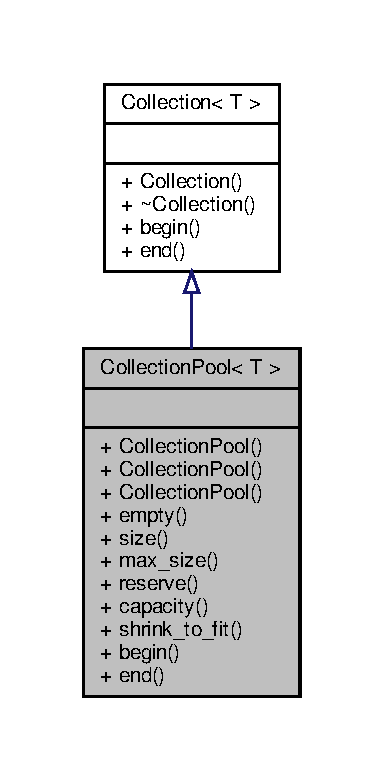
\includegraphics[width=184pt]{class_collection_pool__inherit__graph}
\end{center}
\end{figure}


Graphe de collaboration de Collection\+Pool$<$ T $>$\+:\nopagebreak
\begin{figure}[H]
\begin{center}
\leavevmode
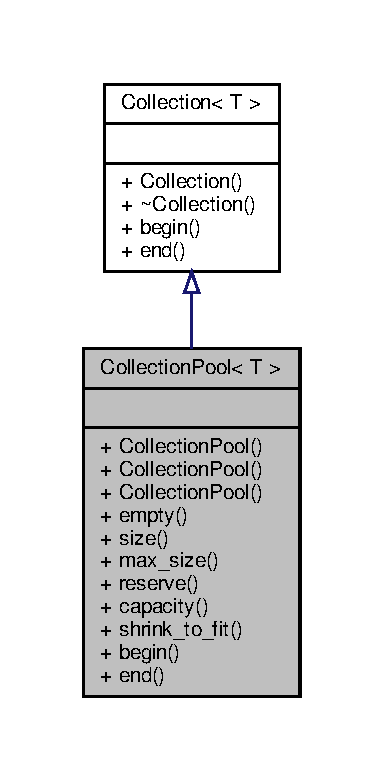
\includegraphics[width=184pt]{class_collection_pool__coll__graph}
\end{center}
\end{figure}
\subsection*{Types publics}
\begin{DoxyCompactItemize}
\item 
using \hyperlink{class_collection_pool_a018a408f2c2bcdf2b542141dbc1d1c17}{value\+\_\+type} = typename \hyperlink{class_collection}{Collection}$<$ T $>$\+::\hyperlink{class_collection_pool_a018a408f2c2bcdf2b542141dbc1d1c17}{value\+\_\+type}
\item 
using \hyperlink{class_collection_pool_a2334b5af86ff5008ec9ad1ff2ea17e19}{allocator\+\_\+type} = typename \hyperlink{class_collection}{Collection}$<$ T $>$\+::\hyperlink{class_collection_ac7974b0b552f0a94065aadc48ae53397}{allocator\+\_\+type}
\item 
using \hyperlink{class_collection_pool_a12dd127db0342d4b694d857f6c77ad90}{reference} = typename \hyperlink{class_collection}{Collection}$<$ T $>$\+::\hyperlink{class_collection_abbc291771b11c48cd2f297a0d9fe0449}{reference}
\item 
using \hyperlink{class_collection_pool_a1861ca0a8e40abe5f8d27ec35fbc439d}{const\+\_\+reference} = typename \hyperlink{class_collection}{Collection}$<$ T $>$\+::\hyperlink{class_collection_abb8c0f6de5e322aa531837aab7358b89}{const\+\_\+reference}
\item 
using \hyperlink{class_collection_pool_a3bfec6c487a93170866fde4b57a85b21}{pointer} = typename \hyperlink{class_collection}{Collection}$<$ T $>$\+::\hyperlink{class_collection_a9a5b5d9b389c113364d527900c745efb}{pointer}
\item 
using \hyperlink{class_collection_pool_ae1a6ed261a58f72a07c40a2cc98325d2}{const\+\_\+pointer} = typename \hyperlink{class_collection}{Collection}$<$ T $>$\+::\hyperlink{class_collection_a79ea96d1fa145e340e907547d0053b81}{const\+\_\+pointer}
\item 
using \hyperlink{class_collection_pool_a7beafeb93ccc043bcde933faab05718f}{iterator} = typename \hyperlink{class_collection}{Collection}$<$ T $>$\+::\hyperlink{class_collection_a317dca4fdf1eb2e47643bb60c620f802}{iterator}
\item 
using \hyperlink{class_collection_pool_a02f041d9c0562d656eaa05a9859780af}{reverse\+\_\+iterator} = typename \hyperlink{class_collection}{Collection}$<$ T $>$\+::\hyperlink{class_collection_ac3805407b2dc537e71db7af070b8d8a6}{reverse\+\_\+iterator}
\item 
using \hyperlink{class_collection_pool_a5e8db21ac58139c891fee4ae87295744}{difference\+\_\+type} = typename \hyperlink{class_collection}{Collection}$<$ T $>$\+::\hyperlink{class_collection_a60b36ef7aba0a88dff0e98fc2adb98a8}{difference\+\_\+type}
\item 
using \hyperlink{class_collection_pool_a3fe4d4cbb79a3cb138cdb3f07c401b00}{size\+\_\+type} = typename \hyperlink{class_collection}{Collection}$<$ T $>$\+::\hyperlink{class_collection_a3f8b024f587aa20be530866da30948c4}{size\+\_\+type}
\end{DoxyCompactItemize}
\subsection*{Fonctions membres publiques}
\begin{DoxyCompactItemize}
\item 
\hyperlink{class_collection_pool_a6e58d0618310fcb2d5114a41c346c1f8}{Collection\+Pool} ()=default
\item 
\hyperlink{class_collection_pool_a65f8fd9c44e03d841391dd50fe953d4a}{Collection\+Pool} (\hyperlink{class_collection_a3f8b024f587aa20be530866da30948c4}{size\+\_\+type} n, const \hyperlink{class_collection_pool_a018a408f2c2bcdf2b542141dbc1d1c17}{value\+\_\+type} \&v=\hyperlink{class_collection_pool_a018a408f2c2bcdf2b542141dbc1d1c17}{value\+\_\+type}\{\})
\item 
\hyperlink{class_collection_pool_a20a624365d44f3b3ae562022d363235b}{Collection\+Pool} (std\+::initializer\+\_\+list$<$ \hyperlink{class_collection_pool_a018a408f2c2bcdf2b542141dbc1d1c17}{value\+\_\+type} $>$ list)
\item 
bool \hyperlink{class_collection_pool_ad73cd0612ec1fd21962f4d423b45b3f6}{empty} () const
\item 
\hyperlink{class_collection_a3f8b024f587aa20be530866da30948c4}{size\+\_\+type} \hyperlink{class_collection_pool_aa5b3ebca322cda930b17a0cfab3f91f2}{size} () const
\item 
\hyperlink{class_collection_a3f8b024f587aa20be530866da30948c4}{size\+\_\+type} \hyperlink{class_collection_pool_a333a1edf4c98229f47b698463baf0324}{max\+\_\+size} () const
\item 
void \hyperlink{class_collection_pool_a06334969f57ca768241af598f03e8de1}{reserve} (\hyperlink{class_collection_a3f8b024f587aa20be530866da30948c4}{size\+\_\+type} new\+\_\+cap)
\item 
\hyperlink{class_collection_a3f8b024f587aa20be530866da30948c4}{size\+\_\+type} \hyperlink{class_collection_pool_a72521883b8761babd44d76a4283d6978}{capacity} () const
\item 
void \hyperlink{class_collection_pool_a99d7be7a85d94c4288683b900af1e087}{shrink\+\_\+to\+\_\+fit} ()
\item 
\hyperlink{class_collection_a317dca4fdf1eb2e47643bb60c620f802}{iterator} \hyperlink{class_collection_pool_ae13d478a26554da9211db064285c7b0b}{begin} () override
\item 
\hyperlink{class_collection_a317dca4fdf1eb2e47643bb60c620f802}{iterator} \hyperlink{class_collection_pool_a870a85422595d6533688704ebe43b520}{end} () override
\end{DoxyCompactItemize}


\subsection{Documentation des définitions de type membres}
\mbox{\Hypertarget{class_collection_pool_a2334b5af86ff5008ec9ad1ff2ea17e19}\label{class_collection_pool_a2334b5af86ff5008ec9ad1ff2ea17e19}} 
\index{Collection\+Pool@{Collection\+Pool}!allocator\+\_\+type@{allocator\+\_\+type}}
\index{allocator\+\_\+type@{allocator\+\_\+type}!Collection\+Pool@{Collection\+Pool}}
\subsubsection{\texorpdfstring{allocator\+\_\+type}{allocator\_type}}
{\footnotesize\ttfamily template$<$typename T $>$ \\
using \hyperlink{class_collection_pool}{Collection\+Pool}$<$ T $>$\+::\hyperlink{class_collection_ac7974b0b552f0a94065aadc48ae53397}{allocator\+\_\+type} =  typename \hyperlink{class_collection}{Collection}$<$T$>$\+::\hyperlink{class_collection_ac7974b0b552f0a94065aadc48ae53397}{allocator\+\_\+type}}

\mbox{\Hypertarget{class_collection_pool_ae1a6ed261a58f72a07c40a2cc98325d2}\label{class_collection_pool_ae1a6ed261a58f72a07c40a2cc98325d2}} 
\index{Collection\+Pool@{Collection\+Pool}!const\+\_\+pointer@{const\+\_\+pointer}}
\index{const\+\_\+pointer@{const\+\_\+pointer}!Collection\+Pool@{Collection\+Pool}}
\subsubsection{\texorpdfstring{const\+\_\+pointer}{const\_pointer}}
{\footnotesize\ttfamily template$<$typename T $>$ \\
using \hyperlink{class_collection_pool}{Collection\+Pool}$<$ T $>$\+::\hyperlink{class_collection_a79ea96d1fa145e340e907547d0053b81}{const\+\_\+pointer} =  typename \hyperlink{class_collection}{Collection}$<$T$>$\+::\hyperlink{class_collection_a79ea96d1fa145e340e907547d0053b81}{const\+\_\+pointer}}

\mbox{\Hypertarget{class_collection_pool_a1861ca0a8e40abe5f8d27ec35fbc439d}\label{class_collection_pool_a1861ca0a8e40abe5f8d27ec35fbc439d}} 
\index{Collection\+Pool@{Collection\+Pool}!const\+\_\+reference@{const\+\_\+reference}}
\index{const\+\_\+reference@{const\+\_\+reference}!Collection\+Pool@{Collection\+Pool}}
\subsubsection{\texorpdfstring{const\+\_\+reference}{const\_reference}}
{\footnotesize\ttfamily template$<$typename T $>$ \\
using \hyperlink{class_collection_pool}{Collection\+Pool}$<$ T $>$\+::\hyperlink{class_collection_abb8c0f6de5e322aa531837aab7358b89}{const\+\_\+reference} =  typename \hyperlink{class_collection}{Collection}$<$T$>$\+::\hyperlink{class_collection_abb8c0f6de5e322aa531837aab7358b89}{const\+\_\+reference}}

\mbox{\Hypertarget{class_collection_pool_a5e8db21ac58139c891fee4ae87295744}\label{class_collection_pool_a5e8db21ac58139c891fee4ae87295744}} 
\index{Collection\+Pool@{Collection\+Pool}!difference\+\_\+type@{difference\+\_\+type}}
\index{difference\+\_\+type@{difference\+\_\+type}!Collection\+Pool@{Collection\+Pool}}
\subsubsection{\texorpdfstring{difference\+\_\+type}{difference\_type}}
{\footnotesize\ttfamily template$<$typename T $>$ \\
using \hyperlink{class_collection_pool}{Collection\+Pool}$<$ T $>$\+::\hyperlink{class_collection_a60b36ef7aba0a88dff0e98fc2adb98a8}{difference\+\_\+type} =  typename \hyperlink{class_collection}{Collection}$<$T$>$\+::\hyperlink{class_collection_a60b36ef7aba0a88dff0e98fc2adb98a8}{difference\+\_\+type}}

\mbox{\Hypertarget{class_collection_pool_a7beafeb93ccc043bcde933faab05718f}\label{class_collection_pool_a7beafeb93ccc043bcde933faab05718f}} 
\index{Collection\+Pool@{Collection\+Pool}!iterator@{iterator}}
\index{iterator@{iterator}!Collection\+Pool@{Collection\+Pool}}
\subsubsection{\texorpdfstring{iterator}{iterator}}
{\footnotesize\ttfamily template$<$typename T $>$ \\
using \hyperlink{class_collection_pool}{Collection\+Pool}$<$ T $>$\+::\hyperlink{class_collection_a317dca4fdf1eb2e47643bb60c620f802}{iterator} =  typename \hyperlink{class_collection}{Collection}$<$T$>$\+::\hyperlink{class_collection_a317dca4fdf1eb2e47643bb60c620f802}{iterator}}

\mbox{\Hypertarget{class_collection_pool_a3bfec6c487a93170866fde4b57a85b21}\label{class_collection_pool_a3bfec6c487a93170866fde4b57a85b21}} 
\index{Collection\+Pool@{Collection\+Pool}!pointer@{pointer}}
\index{pointer@{pointer}!Collection\+Pool@{Collection\+Pool}}
\subsubsection{\texorpdfstring{pointer}{pointer}}
{\footnotesize\ttfamily template$<$typename T $>$ \\
using \hyperlink{class_collection_pool}{Collection\+Pool}$<$ T $>$\+::\hyperlink{class_collection_a9a5b5d9b389c113364d527900c745efb}{pointer} =  typename \hyperlink{class_collection}{Collection}$<$T$>$\+::\hyperlink{class_collection_a9a5b5d9b389c113364d527900c745efb}{pointer}}

\mbox{\Hypertarget{class_collection_pool_a12dd127db0342d4b694d857f6c77ad90}\label{class_collection_pool_a12dd127db0342d4b694d857f6c77ad90}} 
\index{Collection\+Pool@{Collection\+Pool}!reference@{reference}}
\index{reference@{reference}!Collection\+Pool@{Collection\+Pool}}
\subsubsection{\texorpdfstring{reference}{reference}}
{\footnotesize\ttfamily template$<$typename T $>$ \\
using \hyperlink{class_collection_pool}{Collection\+Pool}$<$ T $>$\+::\hyperlink{class_collection_abbc291771b11c48cd2f297a0d9fe0449}{reference} =  typename \hyperlink{class_collection}{Collection}$<$T$>$\+::\hyperlink{class_collection_abbc291771b11c48cd2f297a0d9fe0449}{reference}}

\mbox{\Hypertarget{class_collection_pool_a02f041d9c0562d656eaa05a9859780af}\label{class_collection_pool_a02f041d9c0562d656eaa05a9859780af}} 
\index{Collection\+Pool@{Collection\+Pool}!reverse\+\_\+iterator@{reverse\+\_\+iterator}}
\index{reverse\+\_\+iterator@{reverse\+\_\+iterator}!Collection\+Pool@{Collection\+Pool}}
\subsubsection{\texorpdfstring{reverse\+\_\+iterator}{reverse\_iterator}}
{\footnotesize\ttfamily template$<$typename T $>$ \\
using \hyperlink{class_collection_pool}{Collection\+Pool}$<$ T $>$\+::\hyperlink{class_collection_ac3805407b2dc537e71db7af070b8d8a6}{reverse\+\_\+iterator} =  typename \hyperlink{class_collection}{Collection}$<$T$>$\+::\hyperlink{class_collection_ac3805407b2dc537e71db7af070b8d8a6}{reverse\+\_\+iterator}}

\mbox{\Hypertarget{class_collection_pool_a3fe4d4cbb79a3cb138cdb3f07c401b00}\label{class_collection_pool_a3fe4d4cbb79a3cb138cdb3f07c401b00}} 
\index{Collection\+Pool@{Collection\+Pool}!size\+\_\+type@{size\+\_\+type}}
\index{size\+\_\+type@{size\+\_\+type}!Collection\+Pool@{Collection\+Pool}}
\subsubsection{\texorpdfstring{size\+\_\+type}{size\_type}}
{\footnotesize\ttfamily template$<$typename T $>$ \\
using \hyperlink{class_collection_pool}{Collection\+Pool}$<$ T $>$\+::\hyperlink{class_collection_a3f8b024f587aa20be530866da30948c4}{size\+\_\+type} =  typename \hyperlink{class_collection}{Collection}$<$T$>$\+::\hyperlink{class_collection_a3f8b024f587aa20be530866da30948c4}{size\+\_\+type}}

\mbox{\Hypertarget{class_collection_pool_a018a408f2c2bcdf2b542141dbc1d1c17}\label{class_collection_pool_a018a408f2c2bcdf2b542141dbc1d1c17}} 
\index{Collection\+Pool@{Collection\+Pool}!value\+\_\+type@{value\+\_\+type}}
\index{value\+\_\+type@{value\+\_\+type}!Collection\+Pool@{Collection\+Pool}}
\subsubsection{\texorpdfstring{value\+\_\+type}{value\_type}}
{\footnotesize\ttfamily template$<$typename T $>$ \\
using \hyperlink{class_collection_pool}{Collection\+Pool}$<$ T $>$\+::\hyperlink{class_collection_pool_a018a408f2c2bcdf2b542141dbc1d1c17}{value\+\_\+type} =  typename \hyperlink{class_collection}{Collection}$<$T$>$\+::\hyperlink{class_collection_pool_a018a408f2c2bcdf2b542141dbc1d1c17}{value\+\_\+type}}



\subsection{Documentation des constructeurs et destructeur}
\mbox{\Hypertarget{class_collection_pool_a6e58d0618310fcb2d5114a41c346c1f8}\label{class_collection_pool_a6e58d0618310fcb2d5114a41c346c1f8}} 
\index{Collection\+Pool@{Collection\+Pool}!Collection\+Pool@{Collection\+Pool}}
\index{Collection\+Pool@{Collection\+Pool}!Collection\+Pool@{Collection\+Pool}}
\subsubsection{\texorpdfstring{Collection\+Pool()}{CollectionPool()}\hspace{0.1cm}{\footnotesize\ttfamily [1/3]}}
{\footnotesize\ttfamily template$<$typename T $>$ \\
\hyperlink{class_collection_pool}{Collection\+Pool}$<$ T $>$\+::\hyperlink{class_collection_pool}{Collection\+Pool} (\begin{DoxyParamCaption}{ }\end{DoxyParamCaption})\hspace{0.3cm}{\ttfamily [default]}}

\mbox{\Hypertarget{class_collection_pool_a65f8fd9c44e03d841391dd50fe953d4a}\label{class_collection_pool_a65f8fd9c44e03d841391dd50fe953d4a}} 
\index{Collection\+Pool@{Collection\+Pool}!Collection\+Pool@{Collection\+Pool}}
\index{Collection\+Pool@{Collection\+Pool}!Collection\+Pool@{Collection\+Pool}}
\subsubsection{\texorpdfstring{Collection\+Pool()}{CollectionPool()}\hspace{0.1cm}{\footnotesize\ttfamily [2/3]}}
{\footnotesize\ttfamily template$<$typename T $>$ \\
\hyperlink{class_collection_pool}{Collection\+Pool}$<$ T $>$\+::\hyperlink{class_collection_pool}{Collection\+Pool} (\begin{DoxyParamCaption}\item[{\hyperlink{class_collection_a3f8b024f587aa20be530866da30948c4}{size\+\_\+type}}]{n,  }\item[{const \hyperlink{class_collection_pool_a018a408f2c2bcdf2b542141dbc1d1c17}{value\+\_\+type} \&}]{v = {\ttfamily \hyperlink{class_collection_pool_a018a408f2c2bcdf2b542141dbc1d1c17}{value\+\_\+type}\{\}} }\end{DoxyParamCaption})\hspace{0.3cm}{\ttfamily [inline]}, {\ttfamily [explicit]}}

\mbox{\Hypertarget{class_collection_pool_a20a624365d44f3b3ae562022d363235b}\label{class_collection_pool_a20a624365d44f3b3ae562022d363235b}} 
\index{Collection\+Pool@{Collection\+Pool}!Collection\+Pool@{Collection\+Pool}}
\index{Collection\+Pool@{Collection\+Pool}!Collection\+Pool@{Collection\+Pool}}
\subsubsection{\texorpdfstring{Collection\+Pool()}{CollectionPool()}\hspace{0.1cm}{\footnotesize\ttfamily [3/3]}}
{\footnotesize\ttfamily template$<$typename T $>$ \\
\hyperlink{class_collection_pool}{Collection\+Pool}$<$ T $>$\+::\hyperlink{class_collection_pool}{Collection\+Pool} (\begin{DoxyParamCaption}\item[{std\+::initializer\+\_\+list$<$ \hyperlink{class_collection_pool_a018a408f2c2bcdf2b542141dbc1d1c17}{value\+\_\+type} $>$}]{list }\end{DoxyParamCaption})\hspace{0.3cm}{\ttfamily [inline]}}



\subsection{Documentation des fonctions membres}
\mbox{\Hypertarget{class_collection_pool_ae13d478a26554da9211db064285c7b0b}\label{class_collection_pool_ae13d478a26554da9211db064285c7b0b}} 
\index{Collection\+Pool@{Collection\+Pool}!begin@{begin}}
\index{begin@{begin}!Collection\+Pool@{Collection\+Pool}}
\subsubsection{\texorpdfstring{begin()}{begin()}}
{\footnotesize\ttfamily template$<$typename T $>$ \\
\hyperlink{class_collection_a317dca4fdf1eb2e47643bb60c620f802}{iterator} \hyperlink{class_collection_pool}{Collection\+Pool}$<$ T $>$\+::begin (\begin{DoxyParamCaption}{ }\end{DoxyParamCaption})\hspace{0.3cm}{\ttfamily [inline]}, {\ttfamily [override]}, {\ttfamily [virtual]}}



Implémente \hyperlink{class_collection_a4abc73f8e31a499a22b25d42b7a4fe8c}{Collection$<$ T $>$}.

\mbox{\Hypertarget{class_collection_pool_a72521883b8761babd44d76a4283d6978}\label{class_collection_pool_a72521883b8761babd44d76a4283d6978}} 
\index{Collection\+Pool@{Collection\+Pool}!capacity@{capacity}}
\index{capacity@{capacity}!Collection\+Pool@{Collection\+Pool}}
\subsubsection{\texorpdfstring{capacity()}{capacity()}}
{\footnotesize\ttfamily template$<$typename T $>$ \\
\hyperlink{class_collection_a3f8b024f587aa20be530866da30948c4}{size\+\_\+type} \hyperlink{class_collection_pool}{Collection\+Pool}$<$ T $>$\+::capacity (\begin{DoxyParamCaption}{ }\end{DoxyParamCaption}) const\hspace{0.3cm}{\ttfamily [inline]}}

\mbox{\Hypertarget{class_collection_pool_ad73cd0612ec1fd21962f4d423b45b3f6}\label{class_collection_pool_ad73cd0612ec1fd21962f4d423b45b3f6}} 
\index{Collection\+Pool@{Collection\+Pool}!empty@{empty}}
\index{empty@{empty}!Collection\+Pool@{Collection\+Pool}}
\subsubsection{\texorpdfstring{empty()}{empty()}}
{\footnotesize\ttfamily template$<$typename T $>$ \\
bool \hyperlink{class_collection_pool}{Collection\+Pool}$<$ T $>$\+::empty (\begin{DoxyParamCaption}{ }\end{DoxyParamCaption}) const\hspace{0.3cm}{\ttfamily [inline]}}

\mbox{\Hypertarget{class_collection_pool_a870a85422595d6533688704ebe43b520}\label{class_collection_pool_a870a85422595d6533688704ebe43b520}} 
\index{Collection\+Pool@{Collection\+Pool}!end@{end}}
\index{end@{end}!Collection\+Pool@{Collection\+Pool}}
\subsubsection{\texorpdfstring{end()}{end()}}
{\footnotesize\ttfamily template$<$typename T $>$ \\
\hyperlink{class_collection_a317dca4fdf1eb2e47643bb60c620f802}{iterator} \hyperlink{class_collection_pool}{Collection\+Pool}$<$ T $>$\+::end (\begin{DoxyParamCaption}{ }\end{DoxyParamCaption})\hspace{0.3cm}{\ttfamily [inline]}, {\ttfamily [override]}, {\ttfamily [virtual]}}



Implémente \hyperlink{class_collection_ab5b98f651d0f49cde1be067c69c52e89}{Collection$<$ T $>$}.

\mbox{\Hypertarget{class_collection_pool_a333a1edf4c98229f47b698463baf0324}\label{class_collection_pool_a333a1edf4c98229f47b698463baf0324}} 
\index{Collection\+Pool@{Collection\+Pool}!max\+\_\+size@{max\+\_\+size}}
\index{max\+\_\+size@{max\+\_\+size}!Collection\+Pool@{Collection\+Pool}}
\subsubsection{\texorpdfstring{max\+\_\+size()}{max\_size()}}
{\footnotesize\ttfamily template$<$typename T $>$ \\
\hyperlink{class_collection_a3f8b024f587aa20be530866da30948c4}{size\+\_\+type} \hyperlink{class_collection_pool}{Collection\+Pool}$<$ T $>$\+::max\+\_\+size (\begin{DoxyParamCaption}{ }\end{DoxyParamCaption}) const\hspace{0.3cm}{\ttfamily [inline]}}

\mbox{\Hypertarget{class_collection_pool_a06334969f57ca768241af598f03e8de1}\label{class_collection_pool_a06334969f57ca768241af598f03e8de1}} 
\index{Collection\+Pool@{Collection\+Pool}!reserve@{reserve}}
\index{reserve@{reserve}!Collection\+Pool@{Collection\+Pool}}
\subsubsection{\texorpdfstring{reserve()}{reserve()}}
{\footnotesize\ttfamily template$<$typename T $>$ \\
void \hyperlink{class_collection_pool}{Collection\+Pool}$<$ T $>$\+::reserve (\begin{DoxyParamCaption}\item[{\hyperlink{class_collection_a3f8b024f587aa20be530866da30948c4}{size\+\_\+type}}]{new\+\_\+cap }\end{DoxyParamCaption})\hspace{0.3cm}{\ttfamily [inline]}}

\mbox{\Hypertarget{class_collection_pool_a99d7be7a85d94c4288683b900af1e087}\label{class_collection_pool_a99d7be7a85d94c4288683b900af1e087}} 
\index{Collection\+Pool@{Collection\+Pool}!shrink\+\_\+to\+\_\+fit@{shrink\+\_\+to\+\_\+fit}}
\index{shrink\+\_\+to\+\_\+fit@{shrink\+\_\+to\+\_\+fit}!Collection\+Pool@{Collection\+Pool}}
\subsubsection{\texorpdfstring{shrink\+\_\+to\+\_\+fit()}{shrink\_to\_fit()}}
{\footnotesize\ttfamily template$<$typename T $>$ \\
void \hyperlink{class_collection_pool}{Collection\+Pool}$<$ T $>$\+::shrink\+\_\+to\+\_\+fit (\begin{DoxyParamCaption}{ }\end{DoxyParamCaption})\hspace{0.3cm}{\ttfamily [inline]}}

\mbox{\Hypertarget{class_collection_pool_aa5b3ebca322cda930b17a0cfab3f91f2}\label{class_collection_pool_aa5b3ebca322cda930b17a0cfab3f91f2}} 
\index{Collection\+Pool@{Collection\+Pool}!size@{size}}
\index{size@{size}!Collection\+Pool@{Collection\+Pool}}
\subsubsection{\texorpdfstring{size()}{size()}}
{\footnotesize\ttfamily template$<$typename T $>$ \\
\hyperlink{class_collection_a3f8b024f587aa20be530866da30948c4}{size\+\_\+type} \hyperlink{class_collection_pool}{Collection\+Pool}$<$ T $>$\+::size (\begin{DoxyParamCaption}{ }\end{DoxyParamCaption}) const\hspace{0.3cm}{\ttfamily [inline]}}



La documentation de cette classe a été générée à partir du fichier suivant \+:\begin{DoxyCompactItemize}
\item 
src/\hyperlink{_collection_pool_8hpp}{Collection\+Pool.\+hpp}\end{DoxyCompactItemize}

\hypertarget{class_filtered_collection}{}\section{Référence du modèle de la classe Filtered\+Collection$<$ T $>$}
\label{class_filtered_collection}\index{Filtered\+Collection$<$ T $>$@{Filtered\+Collection$<$ T $>$}}


{\ttfamily \#include $<$Filtered\+Collection.\+hpp$>$}



Graphe d\textquotesingle{}héritage de Filtered\+Collection$<$ T $>$\+:\nopagebreak
\begin{figure}[H]
\begin{center}
\leavevmode
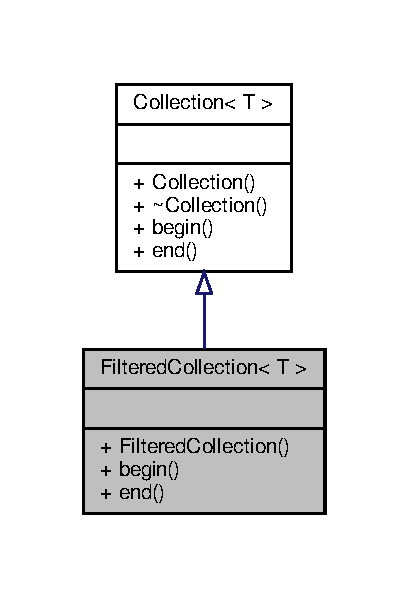
\includegraphics[width=196pt]{class_filtered_collection__inherit__graph}
\end{center}
\end{figure}


Graphe de collaboration de Filtered\+Collection$<$ T $>$\+:\nopagebreak
\begin{figure}[H]
\begin{center}
\leavevmode
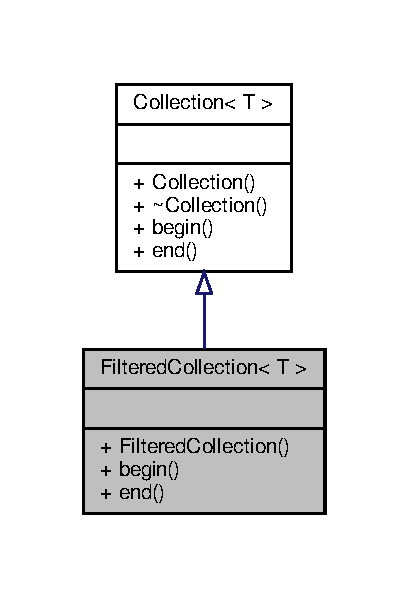
\includegraphics[width=196pt]{class_filtered_collection__coll__graph}
\end{center}
\end{figure}
\subsection*{Types publics}
\begin{DoxyCompactItemize}
\item 
using \hyperlink{class_filtered_collection_a70364ecb37ecfcc313cea1e3dee900da}{value\+\_\+type} = typename \hyperlink{class_collection}{Collection}$<$ T $>$\+::\hyperlink{class_collection_a30ecb2b5696f341f4b751019679c41e0}{value\+\_\+type}
\item 
using \hyperlink{class_filtered_collection_a89348fde51fe48c6528e5ac5abe72c6d}{allocator\+\_\+type} = typename \hyperlink{class_collection}{Collection}$<$ T $>$\+::\hyperlink{class_collection_ac7974b0b552f0a94065aadc48ae53397}{allocator\+\_\+type}
\item 
using \hyperlink{class_filtered_collection_afc4e47695287b6bac73899ab5bcfdf6e}{reference} = typename \hyperlink{class_collection}{Collection}$<$ T $>$\+::\hyperlink{class_collection_abbc291771b11c48cd2f297a0d9fe0449}{reference}
\item 
using \hyperlink{class_filtered_collection_acd1fd308211e928705d0903b749dcaef}{const\+\_\+reference} = typename \hyperlink{class_collection}{Collection}$<$ T $>$\+::\hyperlink{class_collection_abb8c0f6de5e322aa531837aab7358b89}{const\+\_\+reference}
\item 
using \hyperlink{class_filtered_collection_a0c78e02c35e4b712b945a0e5c6b9a14a}{pointer} = typename \hyperlink{class_collection}{Collection}$<$ T $>$\+::\hyperlink{class_collection_a9a5b5d9b389c113364d527900c745efb}{pointer}
\item 
using \hyperlink{class_filtered_collection_af5e238a7b8ed76c864a2c7526b34a71d}{const\+\_\+pointer} = typename \hyperlink{class_collection}{Collection}$<$ T $>$\+::\hyperlink{class_collection_a79ea96d1fa145e340e907547d0053b81}{const\+\_\+pointer}
\item 
using \hyperlink{class_filtered_collection_a65730aaf0a2a5307a924b44672718c74}{iterator} = typename \hyperlink{class_collection}{Collection}$<$ T $>$\+::\hyperlink{class_collection_a317dca4fdf1eb2e47643bb60c620f802}{iterator}
\item 
using \hyperlink{class_filtered_collection_a5b0a5b053f47e55eee9d746d8160664b}{reverse\+\_\+iterator} = typename \hyperlink{class_collection}{Collection}$<$ T $>$\+::\hyperlink{class_collection_ac3805407b2dc537e71db7af070b8d8a6}{reverse\+\_\+iterator}
\item 
using \hyperlink{class_filtered_collection_a98c17401762621a928d2b9926d3b71d6}{difference\+\_\+type} = typename \hyperlink{class_collection}{Collection}$<$ T $>$\+::\hyperlink{class_collection_a60b36ef7aba0a88dff0e98fc2adb98a8}{difference\+\_\+type}
\item 
using \hyperlink{class_filtered_collection_ab527ec70d0bf74af7018c0ca42a6ec8a}{size\+\_\+type} = typename \hyperlink{class_collection}{Collection}$<$ T $>$\+::\hyperlink{class_collection_a3f8b024f587aa20be530866da30948c4}{size\+\_\+type}
\end{DoxyCompactItemize}
\subsection*{Fonctions membres publiques}
\begin{DoxyCompactItemize}
\item 
\hyperlink{class_filtered_collection_a78c712f40560a66d05ce97755d6c0749}{Filtered\+Collection} (\hyperlink{class_collection}{Collection}$<$ T $>$ \&c, const filtre\+\_\+t \&f)
\item 
\hyperlink{class_collection_a317dca4fdf1eb2e47643bb60c620f802}{iterator} \hyperlink{class_filtered_collection_a114f2b1557201e523a264d549926ab0a}{begin} ()
\item 
\hyperlink{class_collection_a317dca4fdf1eb2e47643bb60c620f802}{iterator} \hyperlink{class_filtered_collection_ae310c937df5035ef07f7d4de65fca18b}{end} ()
\end{DoxyCompactItemize}
\subsection*{Amis}
\begin{DoxyCompactItemize}
\item 
class \hyperlink{class_filtered_collection_ac3e52cfdc762d90ccbb2121ff410fc5e}{Filtered\+Iterator$<$ T $>$}
\end{DoxyCompactItemize}


\subsection{Documentation des définitions de type membres}
\mbox{\Hypertarget{class_filtered_collection_a89348fde51fe48c6528e5ac5abe72c6d}\label{class_filtered_collection_a89348fde51fe48c6528e5ac5abe72c6d}} 
\index{Filtered\+Collection@{Filtered\+Collection}!allocator\+\_\+type@{allocator\+\_\+type}}
\index{allocator\+\_\+type@{allocator\+\_\+type}!Filtered\+Collection@{Filtered\+Collection}}
\subsubsection{\texorpdfstring{allocator\+\_\+type}{allocator\_type}}
{\footnotesize\ttfamily template$<$typename T$>$ \\
using \hyperlink{class_filtered_collection}{Filtered\+Collection}$<$ T $>$\+::\hyperlink{class_collection_ac7974b0b552f0a94065aadc48ae53397}{allocator\+\_\+type} =  typename \hyperlink{class_collection}{Collection}$<$T$>$\+::\hyperlink{class_collection_ac7974b0b552f0a94065aadc48ae53397}{allocator\+\_\+type}}

\mbox{\Hypertarget{class_filtered_collection_af5e238a7b8ed76c864a2c7526b34a71d}\label{class_filtered_collection_af5e238a7b8ed76c864a2c7526b34a71d}} 
\index{Filtered\+Collection@{Filtered\+Collection}!const\+\_\+pointer@{const\+\_\+pointer}}
\index{const\+\_\+pointer@{const\+\_\+pointer}!Filtered\+Collection@{Filtered\+Collection}}
\subsubsection{\texorpdfstring{const\+\_\+pointer}{const\_pointer}}
{\footnotesize\ttfamily template$<$typename T$>$ \\
using \hyperlink{class_filtered_collection}{Filtered\+Collection}$<$ T $>$\+::\hyperlink{class_collection_a79ea96d1fa145e340e907547d0053b81}{const\+\_\+pointer} =  typename \hyperlink{class_collection}{Collection}$<$T$>$\+::\hyperlink{class_collection_a79ea96d1fa145e340e907547d0053b81}{const\+\_\+pointer}}

\mbox{\Hypertarget{class_filtered_collection_acd1fd308211e928705d0903b749dcaef}\label{class_filtered_collection_acd1fd308211e928705d0903b749dcaef}} 
\index{Filtered\+Collection@{Filtered\+Collection}!const\+\_\+reference@{const\+\_\+reference}}
\index{const\+\_\+reference@{const\+\_\+reference}!Filtered\+Collection@{Filtered\+Collection}}
\subsubsection{\texorpdfstring{const\+\_\+reference}{const\_reference}}
{\footnotesize\ttfamily template$<$typename T$>$ \\
using \hyperlink{class_filtered_collection}{Filtered\+Collection}$<$ T $>$\+::\hyperlink{class_collection_abb8c0f6de5e322aa531837aab7358b89}{const\+\_\+reference} =  typename \hyperlink{class_collection}{Collection}$<$T$>$\+::\hyperlink{class_collection_abb8c0f6de5e322aa531837aab7358b89}{const\+\_\+reference}}

\mbox{\Hypertarget{class_filtered_collection_a98c17401762621a928d2b9926d3b71d6}\label{class_filtered_collection_a98c17401762621a928d2b9926d3b71d6}} 
\index{Filtered\+Collection@{Filtered\+Collection}!difference\+\_\+type@{difference\+\_\+type}}
\index{difference\+\_\+type@{difference\+\_\+type}!Filtered\+Collection@{Filtered\+Collection}}
\subsubsection{\texorpdfstring{difference\+\_\+type}{difference\_type}}
{\footnotesize\ttfamily template$<$typename T$>$ \\
using \hyperlink{class_filtered_collection}{Filtered\+Collection}$<$ T $>$\+::\hyperlink{class_collection_a60b36ef7aba0a88dff0e98fc2adb98a8}{difference\+\_\+type} =  typename \hyperlink{class_collection}{Collection}$<$T$>$\+::\hyperlink{class_collection_a60b36ef7aba0a88dff0e98fc2adb98a8}{difference\+\_\+type}}

\mbox{\Hypertarget{class_filtered_collection_a65730aaf0a2a5307a924b44672718c74}\label{class_filtered_collection_a65730aaf0a2a5307a924b44672718c74}} 
\index{Filtered\+Collection@{Filtered\+Collection}!iterator@{iterator}}
\index{iterator@{iterator}!Filtered\+Collection@{Filtered\+Collection}}
\subsubsection{\texorpdfstring{iterator}{iterator}}
{\footnotesize\ttfamily template$<$typename T$>$ \\
using \hyperlink{class_filtered_collection}{Filtered\+Collection}$<$ T $>$\+::\hyperlink{class_collection_a317dca4fdf1eb2e47643bb60c620f802}{iterator} =  typename \hyperlink{class_collection}{Collection}$<$T$>$\+::\hyperlink{class_collection_a317dca4fdf1eb2e47643bb60c620f802}{iterator}}

\mbox{\Hypertarget{class_filtered_collection_a0c78e02c35e4b712b945a0e5c6b9a14a}\label{class_filtered_collection_a0c78e02c35e4b712b945a0e5c6b9a14a}} 
\index{Filtered\+Collection@{Filtered\+Collection}!pointer@{pointer}}
\index{pointer@{pointer}!Filtered\+Collection@{Filtered\+Collection}}
\subsubsection{\texorpdfstring{pointer}{pointer}}
{\footnotesize\ttfamily template$<$typename T$>$ \\
using \hyperlink{class_filtered_collection}{Filtered\+Collection}$<$ T $>$\+::\hyperlink{class_collection_a9a5b5d9b389c113364d527900c745efb}{pointer} =  typename \hyperlink{class_collection}{Collection}$<$T$>$\+::\hyperlink{class_collection_a9a5b5d9b389c113364d527900c745efb}{pointer}}

\mbox{\Hypertarget{class_filtered_collection_afc4e47695287b6bac73899ab5bcfdf6e}\label{class_filtered_collection_afc4e47695287b6bac73899ab5bcfdf6e}} 
\index{Filtered\+Collection@{Filtered\+Collection}!reference@{reference}}
\index{reference@{reference}!Filtered\+Collection@{Filtered\+Collection}}
\subsubsection{\texorpdfstring{reference}{reference}}
{\footnotesize\ttfamily template$<$typename T$>$ \\
using \hyperlink{class_filtered_collection}{Filtered\+Collection}$<$ T $>$\+::\hyperlink{class_collection_abbc291771b11c48cd2f297a0d9fe0449}{reference} =  typename \hyperlink{class_collection}{Collection}$<$T$>$\+::\hyperlink{class_collection_abbc291771b11c48cd2f297a0d9fe0449}{reference}}

\mbox{\Hypertarget{class_filtered_collection_a5b0a5b053f47e55eee9d746d8160664b}\label{class_filtered_collection_a5b0a5b053f47e55eee9d746d8160664b}} 
\index{Filtered\+Collection@{Filtered\+Collection}!reverse\+\_\+iterator@{reverse\+\_\+iterator}}
\index{reverse\+\_\+iterator@{reverse\+\_\+iterator}!Filtered\+Collection@{Filtered\+Collection}}
\subsubsection{\texorpdfstring{reverse\+\_\+iterator}{reverse\_iterator}}
{\footnotesize\ttfamily template$<$typename T$>$ \\
using \hyperlink{class_filtered_collection}{Filtered\+Collection}$<$ T $>$\+::\hyperlink{class_collection_ac3805407b2dc537e71db7af070b8d8a6}{reverse\+\_\+iterator} =  typename \hyperlink{class_collection}{Collection}$<$T$>$\+::\hyperlink{class_collection_ac3805407b2dc537e71db7af070b8d8a6}{reverse\+\_\+iterator}}

\mbox{\Hypertarget{class_filtered_collection_ab527ec70d0bf74af7018c0ca42a6ec8a}\label{class_filtered_collection_ab527ec70d0bf74af7018c0ca42a6ec8a}} 
\index{Filtered\+Collection@{Filtered\+Collection}!size\+\_\+type@{size\+\_\+type}}
\index{size\+\_\+type@{size\+\_\+type}!Filtered\+Collection@{Filtered\+Collection}}
\subsubsection{\texorpdfstring{size\+\_\+type}{size\_type}}
{\footnotesize\ttfamily template$<$typename T$>$ \\
using \hyperlink{class_filtered_collection}{Filtered\+Collection}$<$ T $>$\+::\hyperlink{class_collection_a3f8b024f587aa20be530866da30948c4}{size\+\_\+type} =  typename \hyperlink{class_collection}{Collection}$<$T$>$\+::\hyperlink{class_collection_a3f8b024f587aa20be530866da30948c4}{size\+\_\+type}}

\mbox{\Hypertarget{class_filtered_collection_a70364ecb37ecfcc313cea1e3dee900da}\label{class_filtered_collection_a70364ecb37ecfcc313cea1e3dee900da}} 
\index{Filtered\+Collection@{Filtered\+Collection}!value\+\_\+type@{value\+\_\+type}}
\index{value\+\_\+type@{value\+\_\+type}!Filtered\+Collection@{Filtered\+Collection}}
\subsubsection{\texorpdfstring{value\+\_\+type}{value\_type}}
{\footnotesize\ttfamily template$<$typename T$>$ \\
using \hyperlink{class_filtered_collection}{Filtered\+Collection}$<$ T $>$\+::\hyperlink{class_collection_a30ecb2b5696f341f4b751019679c41e0}{value\+\_\+type} =  typename \hyperlink{class_collection}{Collection}$<$T$>$\+::\hyperlink{class_collection_a30ecb2b5696f341f4b751019679c41e0}{value\+\_\+type}}



\subsection{Documentation des constructeurs et destructeur}
\mbox{\Hypertarget{class_filtered_collection_a78c712f40560a66d05ce97755d6c0749}\label{class_filtered_collection_a78c712f40560a66d05ce97755d6c0749}} 
\index{Filtered\+Collection@{Filtered\+Collection}!Filtered\+Collection@{Filtered\+Collection}}
\index{Filtered\+Collection@{Filtered\+Collection}!Filtered\+Collection@{Filtered\+Collection}}
\subsubsection{\texorpdfstring{Filtered\+Collection()}{FilteredCollection()}}
{\footnotesize\ttfamily template$<$typename T$>$ \\
\hyperlink{class_filtered_collection}{Filtered\+Collection}$<$ T $>$\+::\hyperlink{class_filtered_collection}{Filtered\+Collection} (\begin{DoxyParamCaption}\item[{\hyperlink{class_collection}{Collection}$<$ T $>$ \&}]{c,  }\item[{const filtre\+\_\+t \&}]{f }\end{DoxyParamCaption})\hspace{0.3cm}{\ttfamily [inline]}}



\subsection{Documentation des fonctions membres}
\mbox{\Hypertarget{class_filtered_collection_a114f2b1557201e523a264d549926ab0a}\label{class_filtered_collection_a114f2b1557201e523a264d549926ab0a}} 
\index{Filtered\+Collection@{Filtered\+Collection}!begin@{begin}}
\index{begin@{begin}!Filtered\+Collection@{Filtered\+Collection}}
\subsubsection{\texorpdfstring{begin()}{begin()}}
{\footnotesize\ttfamily template$<$typename T$>$ \\
\hyperlink{class_collection_a317dca4fdf1eb2e47643bb60c620f802}{iterator} \hyperlink{class_filtered_collection}{Filtered\+Collection}$<$ T $>$\+::begin (\begin{DoxyParamCaption}{ }\end{DoxyParamCaption})\hspace{0.3cm}{\ttfamily [inline]}, {\ttfamily [virtual]}}



Implémente \hyperlink{class_collection_a4abc73f8e31a499a22b25d42b7a4fe8c}{Collection$<$ T $>$}.



Références Filtered\+Collection$<$ T $>$\+::end().

Voici le graphe d\textquotesingle{}appel pour cette fonction \+:\nopagebreak
\begin{figure}[H]
\begin{center}
\leavevmode
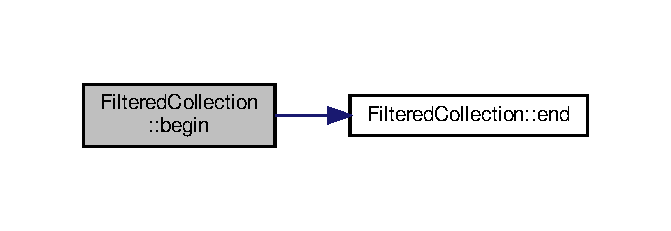
\includegraphics[width=322pt]{class_filtered_collection_a114f2b1557201e523a264d549926ab0a_cgraph}
\end{center}
\end{figure}
\mbox{\Hypertarget{class_filtered_collection_ae310c937df5035ef07f7d4de65fca18b}\label{class_filtered_collection_ae310c937df5035ef07f7d4de65fca18b}} 
\index{Filtered\+Collection@{Filtered\+Collection}!end@{end}}
\index{end@{end}!Filtered\+Collection@{Filtered\+Collection}}
\subsubsection{\texorpdfstring{end()}{end()}}
{\footnotesize\ttfamily template$<$typename T$>$ \\
\hyperlink{class_collection_a317dca4fdf1eb2e47643bb60c620f802}{iterator} \hyperlink{class_filtered_collection}{Filtered\+Collection}$<$ T $>$\+::end (\begin{DoxyParamCaption}{ }\end{DoxyParamCaption})\hspace{0.3cm}{\ttfamily [inline]}, {\ttfamily [virtual]}}



Implémente \hyperlink{class_collection_ab5b98f651d0f49cde1be067c69c52e89}{Collection$<$ T $>$}.



Référencé par Filtered\+Collection$<$ T $>$\+::begin().

Voici le graphe des appelants de cette fonction \+:\nopagebreak
\begin{figure}[H]
\begin{center}
\leavevmode
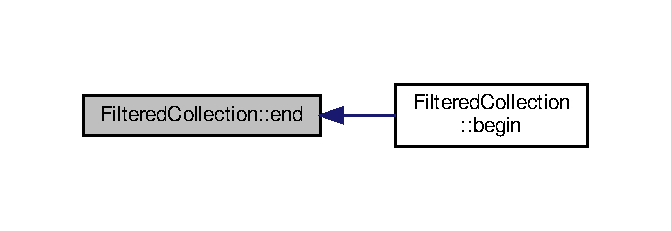
\includegraphics[width=322pt]{class_filtered_collection_ae310c937df5035ef07f7d4de65fca18b_icgraph}
\end{center}
\end{figure}


\subsection{Documentation des fonctions amies et associées}
\mbox{\Hypertarget{class_filtered_collection_ac3e52cfdc762d90ccbb2121ff410fc5e}\label{class_filtered_collection_ac3e52cfdc762d90ccbb2121ff410fc5e}} 
\index{Filtered\+Collection@{Filtered\+Collection}!Filtered\+Iterator$<$ T $>$@{Filtered\+Iterator$<$ T $>$}}
\index{Filtered\+Iterator$<$ T $>$@{Filtered\+Iterator$<$ T $>$}!Filtered\+Collection@{Filtered\+Collection}}
\subsubsection{\texorpdfstring{Filtered\+Iterator$<$ T $>$}{FilteredIterator< T >}}
{\footnotesize\ttfamily template$<$typename T$>$ \\
friend class \hyperlink{class_filtered_iterator}{Filtered\+Iterator}$<$ T $>$\hspace{0.3cm}{\ttfamily [friend]}}



La documentation de cette classe a été générée à partir du fichier suivant \+:\begin{DoxyCompactItemize}
\item 
src/\hyperlink{_filtered_collection_8hpp}{Filtered\+Collection.\+hpp}\end{DoxyCompactItemize}

\hypertarget{class_filtered_iterator}{}\section{Référence du modèle de la classe Filtered\+Iterator$<$ T $>$}
\label{class_filtered_iterator}\index{Filtered\+Iterator$<$ T $>$@{Filtered\+Iterator$<$ T $>$}}


{\ttfamily \#include $<$Filtered\+Collection.\+hpp$>$}



Graphe d\textquotesingle{}héritage de Filtered\+Iterator$<$ T $>$\+:\nopagebreak
\begin{figure}[H]
\begin{center}
\leavevmode
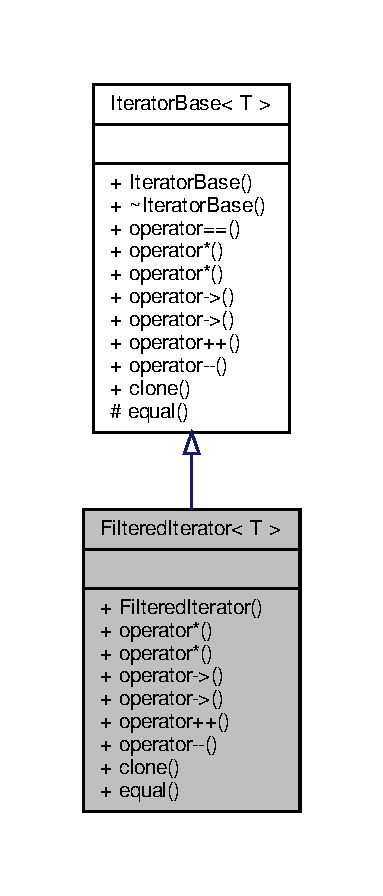
\includegraphics[width=184pt]{class_filtered_iterator__inherit__graph}
\end{center}
\end{figure}


Graphe de collaboration de Filtered\+Iterator$<$ T $>$\+:\nopagebreak
\begin{figure}[H]
\begin{center}
\leavevmode
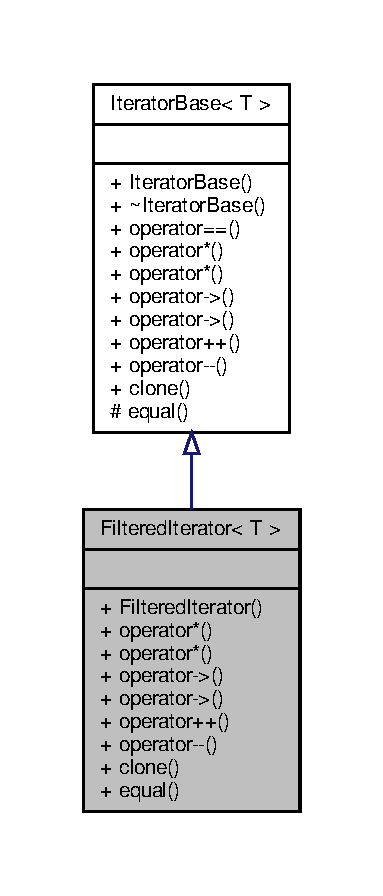
\includegraphics[width=184pt]{class_filtered_iterator__coll__graph}
\end{center}
\end{figure}
\subsection*{Fonctions membres publiques}
\begin{DoxyCompactItemize}
\item 
\hyperlink{class_filtered_iterator_a7d4de1fd089da50804d41dcf387b5e4e}{Filtered\+Iterator} (\hyperlink{class_filtered_collection}{Filtered\+Collection}$<$ T $>$ \&f, \hyperlink{class_collection_iterator}{Collection\+Iterator}$<$ T $>$ itr, bool valid=true)
\item 
T \& \hyperlink{class_filtered_iterator_ac891b168cd653612ddc7ed7cb4380196}{operator$\ast$} () override
\item 
const T \& \hyperlink{class_filtered_iterator_aab76ce411b72c85c3e6a9007a6c9fd98}{operator$\ast$} () const override
\item 
T $\ast$ \hyperlink{class_filtered_iterator_a413726d7cc9a951d0a30eaee6cf36de1}{operator-\/$>$} () override
\item 
const T $\ast$ \hyperlink{class_filtered_iterator_a75ea4ec86c45f496c1515e8e9832cd0f}{operator-\/$>$} () const override
\item 
void \hyperlink{class_filtered_iterator_ae31347c47637172be3d19dc3be30f5cc}{operator++} () override
\item 
void \hyperlink{class_filtered_iterator_a860a37fdf31e87a96b80cb295e6d34c2}{operator-\/-\/} () override
\item 
\hyperlink{class_iterator_base}{Iterator\+Base}$<$ T $>$ $\ast$ \hyperlink{class_filtered_iterator_a79d512a43aa4d31caf26908e93130b9d}{clone} () const override
\item 
bool \hyperlink{class_filtered_iterator_a7118ec2bba2bf138ca771a394a8d72c8}{equal} (const \hyperlink{class_iterator_base}{Iterator\+Base}$<$ T $>$ \&rhs) const override
\end{DoxyCompactItemize}
\subsection*{Membres hérités additionnels}


\subsection{Documentation des constructeurs et destructeur}
\mbox{\Hypertarget{class_filtered_iterator_a7d4de1fd089da50804d41dcf387b5e4e}\label{class_filtered_iterator_a7d4de1fd089da50804d41dcf387b5e4e}} 
\index{Filtered\+Iterator@{Filtered\+Iterator}!Filtered\+Iterator@{Filtered\+Iterator}}
\index{Filtered\+Iterator@{Filtered\+Iterator}!Filtered\+Iterator@{Filtered\+Iterator}}
\subsubsection{\texorpdfstring{Filtered\+Iterator()}{FilteredIterator()}}
{\footnotesize\ttfamily template$<$typename T $>$ \\
\hyperlink{class_filtered_iterator}{Filtered\+Iterator}$<$ T $>$\+::\hyperlink{class_filtered_iterator}{Filtered\+Iterator} (\begin{DoxyParamCaption}\item[{\hyperlink{class_filtered_collection}{Filtered\+Collection}$<$ T $>$ \&}]{f,  }\item[{\hyperlink{class_collection_iterator}{Collection\+Iterator}$<$ T $>$}]{itr,  }\item[{bool}]{valid = {\ttfamily true} }\end{DoxyParamCaption})\hspace{0.3cm}{\ttfamily [inline]}}



\subsection{Documentation des fonctions membres}
\mbox{\Hypertarget{class_filtered_iterator_a79d512a43aa4d31caf26908e93130b9d}\label{class_filtered_iterator_a79d512a43aa4d31caf26908e93130b9d}} 
\index{Filtered\+Iterator@{Filtered\+Iterator}!clone@{clone}}
\index{clone@{clone}!Filtered\+Iterator@{Filtered\+Iterator}}
\subsubsection{\texorpdfstring{clone()}{clone()}}
{\footnotesize\ttfamily template$<$typename T $>$ \\
\hyperlink{class_iterator_base}{Iterator\+Base}$<$T$>$$\ast$ \hyperlink{class_filtered_iterator}{Filtered\+Iterator}$<$ T $>$\+::clone (\begin{DoxyParamCaption}{ }\end{DoxyParamCaption}) const\hspace{0.3cm}{\ttfamily [inline]}, {\ttfamily [override]}, {\ttfamily [virtual]}}



Implémente \hyperlink{class_iterator_base_a541fdf8cc48f31c8ddfdc3f319a37100}{Iterator\+Base$<$ T $>$}.

\mbox{\Hypertarget{class_filtered_iterator_a7118ec2bba2bf138ca771a394a8d72c8}\label{class_filtered_iterator_a7118ec2bba2bf138ca771a394a8d72c8}} 
\index{Filtered\+Iterator@{Filtered\+Iterator}!equal@{equal}}
\index{equal@{equal}!Filtered\+Iterator@{Filtered\+Iterator}}
\subsubsection{\texorpdfstring{equal()}{equal()}}
{\footnotesize\ttfamily template$<$typename T $>$ \\
bool \hyperlink{class_filtered_iterator}{Filtered\+Iterator}$<$ T $>$\+::equal (\begin{DoxyParamCaption}\item[{const \hyperlink{class_iterator_base}{Iterator\+Base}$<$ T $>$ \&}]{rhs }\end{DoxyParamCaption}) const\hspace{0.3cm}{\ttfamily [inline]}, {\ttfamily [override]}, {\ttfamily [virtual]}}



Implémente \hyperlink{class_iterator_base_a08430515a17384d098eb62ecce1b64c6}{Iterator\+Base$<$ T $>$}.

\mbox{\Hypertarget{class_filtered_iterator_ac891b168cd653612ddc7ed7cb4380196}\label{class_filtered_iterator_ac891b168cd653612ddc7ed7cb4380196}} 
\index{Filtered\+Iterator@{Filtered\+Iterator}!operator$\ast$@{operator$\ast$}}
\index{operator$\ast$@{operator$\ast$}!Filtered\+Iterator@{Filtered\+Iterator}}
\subsubsection{\texorpdfstring{operator$\ast$()}{operator*()}\hspace{0.1cm}{\footnotesize\ttfamily [1/2]}}
{\footnotesize\ttfamily template$<$typename T $>$ \\
T\& \hyperlink{class_filtered_iterator}{Filtered\+Iterator}$<$ T $>$\+::operator$\ast$ (\begin{DoxyParamCaption}{ }\end{DoxyParamCaption})\hspace{0.3cm}{\ttfamily [inline]}, {\ttfamily [override]}, {\ttfamily [virtual]}}



Implémente \hyperlink{class_iterator_base_a532583e58bce168648bdbdedb3a7d5ab}{Iterator\+Base$<$ T $>$}.

\mbox{\Hypertarget{class_filtered_iterator_aab76ce411b72c85c3e6a9007a6c9fd98}\label{class_filtered_iterator_aab76ce411b72c85c3e6a9007a6c9fd98}} 
\index{Filtered\+Iterator@{Filtered\+Iterator}!operator$\ast$@{operator$\ast$}}
\index{operator$\ast$@{operator$\ast$}!Filtered\+Iterator@{Filtered\+Iterator}}
\subsubsection{\texorpdfstring{operator$\ast$()}{operator*()}\hspace{0.1cm}{\footnotesize\ttfamily [2/2]}}
{\footnotesize\ttfamily template$<$typename T $>$ \\
const T\& \hyperlink{class_filtered_iterator}{Filtered\+Iterator}$<$ T $>$\+::operator$\ast$ (\begin{DoxyParamCaption}{ }\end{DoxyParamCaption}) const\hspace{0.3cm}{\ttfamily [inline]}, {\ttfamily [override]}, {\ttfamily [virtual]}}



Implémente \hyperlink{class_iterator_base_abc219468b68f2b5471494d04d00f6ec7}{Iterator\+Base$<$ T $>$}.

\mbox{\Hypertarget{class_filtered_iterator_ae31347c47637172be3d19dc3be30f5cc}\label{class_filtered_iterator_ae31347c47637172be3d19dc3be30f5cc}} 
\index{Filtered\+Iterator@{Filtered\+Iterator}!operator++@{operator++}}
\index{operator++@{operator++}!Filtered\+Iterator@{Filtered\+Iterator}}
\subsubsection{\texorpdfstring{operator++()}{operator++()}}
{\footnotesize\ttfamily template$<$typename T $>$ \\
void \hyperlink{class_filtered_iterator}{Filtered\+Iterator}$<$ T $>$\+::operator++ (\begin{DoxyParamCaption}{ }\end{DoxyParamCaption})\hspace{0.3cm}{\ttfamily [inline]}, {\ttfamily [override]}, {\ttfamily [virtual]}}



Implémente \hyperlink{class_iterator_base_a816f35e9020716d212124a34f1c033fb}{Iterator\+Base$<$ T $>$}.

\mbox{\Hypertarget{class_filtered_iterator_a860a37fdf31e87a96b80cb295e6d34c2}\label{class_filtered_iterator_a860a37fdf31e87a96b80cb295e6d34c2}} 
\index{Filtered\+Iterator@{Filtered\+Iterator}!operator-\/-\/@{operator-\/-\/}}
\index{operator-\/-\/@{operator-\/-\/}!Filtered\+Iterator@{Filtered\+Iterator}}
\subsubsection{\texorpdfstring{operator-\/-\/()}{operator--()}}
{\footnotesize\ttfamily template$<$typename T $>$ \\
void \hyperlink{class_filtered_iterator}{Filtered\+Iterator}$<$ T $>$\+::operator-\/-\/ (\begin{DoxyParamCaption}{ }\end{DoxyParamCaption})\hspace{0.3cm}{\ttfamily [inline]}, {\ttfamily [override]}, {\ttfamily [virtual]}}



Implémente \hyperlink{class_iterator_base_aa9bf0f75a8bb7e4d416a9b88ccacd9c7}{Iterator\+Base$<$ T $>$}.

\mbox{\Hypertarget{class_filtered_iterator_a413726d7cc9a951d0a30eaee6cf36de1}\label{class_filtered_iterator_a413726d7cc9a951d0a30eaee6cf36de1}} 
\index{Filtered\+Iterator@{Filtered\+Iterator}!operator-\/$>$@{operator-\/$>$}}
\index{operator-\/$>$@{operator-\/$>$}!Filtered\+Iterator@{Filtered\+Iterator}}
\subsubsection{\texorpdfstring{operator-\/$>$()}{operator->()}\hspace{0.1cm}{\footnotesize\ttfamily [1/2]}}
{\footnotesize\ttfamily template$<$typename T $>$ \\
T$\ast$ \hyperlink{class_filtered_iterator}{Filtered\+Iterator}$<$ T $>$\+::operator-\/$>$ (\begin{DoxyParamCaption}{ }\end{DoxyParamCaption})\hspace{0.3cm}{\ttfamily [inline]}, {\ttfamily [override]}, {\ttfamily [virtual]}}



Implémente \hyperlink{class_iterator_base_aad2254f7877e4647f699ceb455e893ff}{Iterator\+Base$<$ T $>$}.

\mbox{\Hypertarget{class_filtered_iterator_a75ea4ec86c45f496c1515e8e9832cd0f}\label{class_filtered_iterator_a75ea4ec86c45f496c1515e8e9832cd0f}} 
\index{Filtered\+Iterator@{Filtered\+Iterator}!operator-\/$>$@{operator-\/$>$}}
\index{operator-\/$>$@{operator-\/$>$}!Filtered\+Iterator@{Filtered\+Iterator}}
\subsubsection{\texorpdfstring{operator-\/$>$()}{operator->()}\hspace{0.1cm}{\footnotesize\ttfamily [2/2]}}
{\footnotesize\ttfamily template$<$typename T $>$ \\
const T$\ast$ \hyperlink{class_filtered_iterator}{Filtered\+Iterator}$<$ T $>$\+::operator-\/$>$ (\begin{DoxyParamCaption}{ }\end{DoxyParamCaption}) const\hspace{0.3cm}{\ttfamily [inline]}, {\ttfamily [override]}, {\ttfamily [virtual]}}



Implémente \hyperlink{class_iterator_base_a49d96fd63062ca0d7fd813517ad69f03}{Iterator\+Base$<$ T $>$}.



La documentation de cette classe a été générée à partir du fichier suivant \+:\begin{DoxyCompactItemize}
\item 
src/\hyperlink{_filtered_collection_8hpp}{Filtered\+Collection.\+hpp}\end{DoxyCompactItemize}

\hypertarget{class_image}{}\section{Référence du modèle de la classe Image$<$ img\+\_\+t $>$}
\label{class_image}\index{Image$<$ img\+\_\+t $>$@{Image$<$ img\+\_\+t $>$}}


{\ttfamily \#include $<$Image.\+hpp$>$}



Graphe de collaboration de Image$<$ img\+\_\+t $>$\+:\nopagebreak
\begin{figure}[H]
\begin{center}
\leavevmode
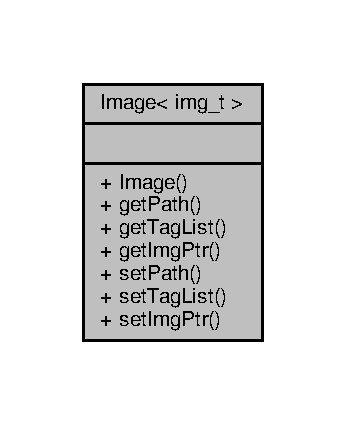
\includegraphics[width=166pt]{class_image__coll__graph}
\end{center}
\end{figure}
\subsection*{Fonctions membres publiques}
\begin{DoxyCompactItemize}
\item 
\hyperlink{class_image_abc511289078a75b6565adaa1c697b2b8}{Image} (std\+::experimental\+::filesystem\+::path p, std\+::unique\+\_\+ptr$<$ img\+\_\+t $>$ img\+Ptr=nullptr, \hyperlink{_tag_list_8hpp_ac0222328791bb6c859b87ac65d5e9f65}{Tag\+List} t=\{\})
\item 
std\+::experimental\+::filesystem\+::path \hyperlink{class_image_a0f940439733c6b4e65f192400119e6d2}{get\+Path} ()
\item 
\hyperlink{_tag_list_8hpp_ac0222328791bb6c859b87ac65d5e9f65}{Tag\+List} \hyperlink{class_image_a35c662168b7b44e9372993691d422ad2}{get\+Tag\+List} ()
\item 
img\+\_\+t $\ast$ \hyperlink{class_image_a368ba28239858cff26afe25c0101d7bb}{get\+Img\+Ptr} ()
\item 
void \hyperlink{class_image_ad7a712265f2243a3292e763b964110b8}{set\+Path} (std\+::experimental\+::filesystem\+::path p)
\item 
void \hyperlink{class_image_a33cfdb0bb6a86aa10fa1f9bf62dbb236}{set\+Tag\+List} (\hyperlink{_tag_list_8hpp_ac0222328791bb6c859b87ac65d5e9f65}{Tag\+List} t)
\item 
void \hyperlink{class_image_aa21c33b7da565d5b4576c5e56ba08cac}{set\+Img\+Ptr} (img\+\_\+t $\ast$img\+Ptr)
\end{DoxyCompactItemize}


\subsection{Documentation des constructeurs et destructeur}
\mbox{\Hypertarget{class_image_abc511289078a75b6565adaa1c697b2b8}\label{class_image_abc511289078a75b6565adaa1c697b2b8}} 
\index{Image@{Image}!Image@{Image}}
\index{Image@{Image}!Image@{Image}}
\subsubsection{\texorpdfstring{Image()}{Image()}}
{\footnotesize\ttfamily template$<$typename img\+\_\+t$>$ \\
\hyperlink{class_image}{Image}$<$ img\+\_\+t $>$\+::\hyperlink{class_image}{Image} (\begin{DoxyParamCaption}\item[{std\+::experimental\+::filesystem\+::path}]{p,  }\item[{std\+::unique\+\_\+ptr$<$ img\+\_\+t $>$}]{img\+Ptr = {\ttfamily nullptr},  }\item[{\hyperlink{_tag_list_8hpp_ac0222328791bb6c859b87ac65d5e9f65}{Tag\+List}}]{t = {\ttfamily \{\}} }\end{DoxyParamCaption})\hspace{0.3cm}{\ttfamily [inline]}}



\subsection{Documentation des fonctions membres}
\mbox{\Hypertarget{class_image_a368ba28239858cff26afe25c0101d7bb}\label{class_image_a368ba28239858cff26afe25c0101d7bb}} 
\index{Image@{Image}!get\+Img\+Ptr@{get\+Img\+Ptr}}
\index{get\+Img\+Ptr@{get\+Img\+Ptr}!Image@{Image}}
\subsubsection{\texorpdfstring{get\+Img\+Ptr()}{getImgPtr()}}
{\footnotesize\ttfamily template$<$typename img\+\_\+t$>$ \\
img\+\_\+t$\ast$ \hyperlink{class_image}{Image}$<$ img\+\_\+t $>$\+::get\+Img\+Ptr (\begin{DoxyParamCaption}{ }\end{DoxyParamCaption})\hspace{0.3cm}{\ttfamily [inline]}}

\mbox{\Hypertarget{class_image_a0f940439733c6b4e65f192400119e6d2}\label{class_image_a0f940439733c6b4e65f192400119e6d2}} 
\index{Image@{Image}!get\+Path@{get\+Path}}
\index{get\+Path@{get\+Path}!Image@{Image}}
\subsubsection{\texorpdfstring{get\+Path()}{getPath()}}
{\footnotesize\ttfamily template$<$typename img\+\_\+t$>$ \\
std\+::experimental\+::filesystem\+::path \hyperlink{class_image}{Image}$<$ img\+\_\+t $>$\+::get\+Path (\begin{DoxyParamCaption}{ }\end{DoxyParamCaption})\hspace{0.3cm}{\ttfamily [inline]}}

\mbox{\Hypertarget{class_image_a35c662168b7b44e9372993691d422ad2}\label{class_image_a35c662168b7b44e9372993691d422ad2}} 
\index{Image@{Image}!get\+Tag\+List@{get\+Tag\+List}}
\index{get\+Tag\+List@{get\+Tag\+List}!Image@{Image}}
\subsubsection{\texorpdfstring{get\+Tag\+List()}{getTagList()}}
{\footnotesize\ttfamily template$<$typename img\+\_\+t$>$ \\
\hyperlink{_tag_list_8hpp_ac0222328791bb6c859b87ac65d5e9f65}{Tag\+List} \hyperlink{class_image}{Image}$<$ img\+\_\+t $>$\+::get\+Tag\+List (\begin{DoxyParamCaption}{ }\end{DoxyParamCaption})\hspace{0.3cm}{\ttfamily [inline]}}

\mbox{\Hypertarget{class_image_aa21c33b7da565d5b4576c5e56ba08cac}\label{class_image_aa21c33b7da565d5b4576c5e56ba08cac}} 
\index{Image@{Image}!set\+Img\+Ptr@{set\+Img\+Ptr}}
\index{set\+Img\+Ptr@{set\+Img\+Ptr}!Image@{Image}}
\subsubsection{\texorpdfstring{set\+Img\+Ptr()}{setImgPtr()}}
{\footnotesize\ttfamily template$<$typename img\+\_\+t$>$ \\
void \hyperlink{class_image}{Image}$<$ img\+\_\+t $>$\+::set\+Img\+Ptr (\begin{DoxyParamCaption}\item[{img\+\_\+t $\ast$}]{img\+Ptr }\end{DoxyParamCaption})\hspace{0.3cm}{\ttfamily [inline]}}

\mbox{\Hypertarget{class_image_ad7a712265f2243a3292e763b964110b8}\label{class_image_ad7a712265f2243a3292e763b964110b8}} 
\index{Image@{Image}!set\+Path@{set\+Path}}
\index{set\+Path@{set\+Path}!Image@{Image}}
\subsubsection{\texorpdfstring{set\+Path()}{setPath()}}
{\footnotesize\ttfamily template$<$typename img\+\_\+t$>$ \\
void \hyperlink{class_image}{Image}$<$ img\+\_\+t $>$\+::set\+Path (\begin{DoxyParamCaption}\item[{std\+::experimental\+::filesystem\+::path}]{p }\end{DoxyParamCaption})\hspace{0.3cm}{\ttfamily [inline]}}

\mbox{\Hypertarget{class_image_a33cfdb0bb6a86aa10fa1f9bf62dbb236}\label{class_image_a33cfdb0bb6a86aa10fa1f9bf62dbb236}} 
\index{Image@{Image}!set\+Tag\+List@{set\+Tag\+List}}
\index{set\+Tag\+List@{set\+Tag\+List}!Image@{Image}}
\subsubsection{\texorpdfstring{set\+Tag\+List()}{setTagList()}}
{\footnotesize\ttfamily template$<$typename img\+\_\+t$>$ \\
void \hyperlink{class_image}{Image}$<$ img\+\_\+t $>$\+::set\+Tag\+List (\begin{DoxyParamCaption}\item[{\hyperlink{_tag_list_8hpp_ac0222328791bb6c859b87ac65d5e9f65}{Tag\+List}}]{t }\end{DoxyParamCaption})\hspace{0.3cm}{\ttfamily [inline]}}



La documentation de cette classe a été générée à partir du fichier suivant \+:\begin{DoxyCompactItemize}
\item 
src/\hyperlink{_image_8hpp}{Image.\+hpp}\end{DoxyCompactItemize}

\hypertarget{class_iterator_base}{}\section{Référence du modèle de la classe Iterator\+Base$<$ T $>$}
\label{class_iterator_base}\index{Iterator\+Base$<$ T $>$@{Iterator\+Base$<$ T $>$}}


{\ttfamily \#include $<$Collection\+Iterator.\+hpp$>$}



Graphe d\textquotesingle{}héritage de Iterator\+Base$<$ T $>$\+:\nopagebreak
\begin{figure}[H]
\begin{center}
\leavevmode
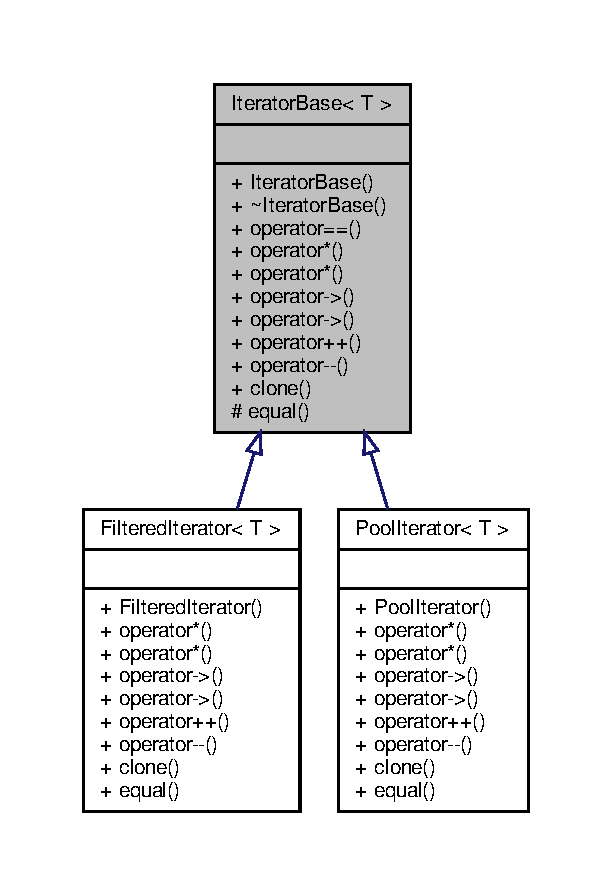
\includegraphics[width=294pt]{class_iterator_base__inherit__graph}
\end{center}
\end{figure}


Graphe de collaboration de Iterator\+Base$<$ T $>$\+:\nopagebreak
\begin{figure}[H]
\begin{center}
\leavevmode
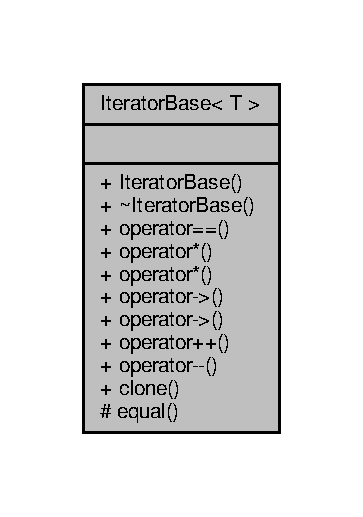
\includegraphics[width=174pt]{class_iterator_base__coll__graph}
\end{center}
\end{figure}
\subsection*{Fonctions membres publiques}
\begin{DoxyCompactItemize}
\item 
\hyperlink{class_iterator_base_a6d1810e7a0a84574bb61d78bb99d96bb}{Iterator\+Base} ()=default
\item 
virtual \hyperlink{class_iterator_base_a9b0e1d44c1fb3e68171746b045676526}{$\sim$\+Iterator\+Base} ()=default
\item 
bool \hyperlink{class_iterator_base_a7475728422cb73f91d1c4cb4c3d07499}{operator==} (const \hyperlink{class_iterator_base}{Iterator\+Base} \&rhs) const
\item 
virtual T \& \hyperlink{class_iterator_base_a532583e58bce168648bdbdedb3a7d5ab}{operator$\ast$} ()=0
\item 
virtual const T \& \hyperlink{class_iterator_base_abc219468b68f2b5471494d04d00f6ec7}{operator$\ast$} () const =0
\item 
virtual T $\ast$ \hyperlink{class_iterator_base_aad2254f7877e4647f699ceb455e893ff}{operator-\/$>$} ()=0
\item 
virtual const T $\ast$ \hyperlink{class_iterator_base_a49d96fd63062ca0d7fd813517ad69f03}{operator-\/$>$} () const =0
\item 
virtual void \hyperlink{class_iterator_base_a816f35e9020716d212124a34f1c033fb}{operator++} ()=0
\item 
virtual void \hyperlink{class_iterator_base_aa9bf0f75a8bb7e4d416a9b88ccacd9c7}{operator-\/-\/} ()=0
\item 
virtual \hyperlink{class_iterator_base}{Iterator\+Base} $\ast$ \hyperlink{class_iterator_base_a541fdf8cc48f31c8ddfdc3f319a37100}{clone} () const =0
\end{DoxyCompactItemize}
\subsection*{Fonctions membres protégées}
\begin{DoxyCompactItemize}
\item 
virtual bool \hyperlink{class_iterator_base_a08430515a17384d098eb62ecce1b64c6}{equal} (const \hyperlink{class_iterator_base}{Iterator\+Base} \&rhs) const =0
\end{DoxyCompactItemize}


\subsection{Documentation des constructeurs et destructeur}
\mbox{\Hypertarget{class_iterator_base_a6d1810e7a0a84574bb61d78bb99d96bb}\label{class_iterator_base_a6d1810e7a0a84574bb61d78bb99d96bb}} 
\index{Iterator\+Base@{Iterator\+Base}!Iterator\+Base@{Iterator\+Base}}
\index{Iterator\+Base@{Iterator\+Base}!Iterator\+Base@{Iterator\+Base}}
\subsubsection{\texorpdfstring{Iterator\+Base()}{IteratorBase()}}
{\footnotesize\ttfamily template$<$typename T$>$ \\
\hyperlink{class_iterator_base}{Iterator\+Base}$<$ T $>$\+::\hyperlink{class_iterator_base}{Iterator\+Base} (\begin{DoxyParamCaption}{ }\end{DoxyParamCaption})\hspace{0.3cm}{\ttfamily [default]}}

\mbox{\Hypertarget{class_iterator_base_a9b0e1d44c1fb3e68171746b045676526}\label{class_iterator_base_a9b0e1d44c1fb3e68171746b045676526}} 
\index{Iterator\+Base@{Iterator\+Base}!````~Iterator\+Base@{$\sim$\+Iterator\+Base}}
\index{````~Iterator\+Base@{$\sim$\+Iterator\+Base}!Iterator\+Base@{Iterator\+Base}}
\subsubsection{\texorpdfstring{$\sim$\+Iterator\+Base()}{~IteratorBase()}}
{\footnotesize\ttfamily template$<$typename T$>$ \\
virtual \hyperlink{class_iterator_base}{Iterator\+Base}$<$ T $>$\+::$\sim$\hyperlink{class_iterator_base}{Iterator\+Base} (\begin{DoxyParamCaption}{ }\end{DoxyParamCaption})\hspace{0.3cm}{\ttfamily [virtual]}, {\ttfamily [default]}}



\subsection{Documentation des fonctions membres}
\mbox{\Hypertarget{class_iterator_base_a541fdf8cc48f31c8ddfdc3f319a37100}\label{class_iterator_base_a541fdf8cc48f31c8ddfdc3f319a37100}} 
\index{Iterator\+Base@{Iterator\+Base}!clone@{clone}}
\index{clone@{clone}!Iterator\+Base@{Iterator\+Base}}
\subsubsection{\texorpdfstring{clone()}{clone()}}
{\footnotesize\ttfamily template$<$typename T$>$ \\
virtual \hyperlink{class_iterator_base}{Iterator\+Base}$\ast$ \hyperlink{class_iterator_base}{Iterator\+Base}$<$ T $>$\+::clone (\begin{DoxyParamCaption}{ }\end{DoxyParamCaption}) const\hspace{0.3cm}{\ttfamily [pure virtual]}}



Implémenté dans \hyperlink{class_filtered_iterator_a79d512a43aa4d31caf26908e93130b9d}{Filtered\+Iterator$<$ T $>$}, et \hyperlink{class_pool_iterator_ae39cdb4bbb84e88cf0d9009e7bdae586}{Pool\+Iterator$<$ T $>$}.



Référencé par Iterator\+Base$<$ T $>$\+::operator==().

Voici le graphe des appelants de cette fonction \+:\nopagebreak
\begin{figure}[H]
\begin{center}
\leavevmode
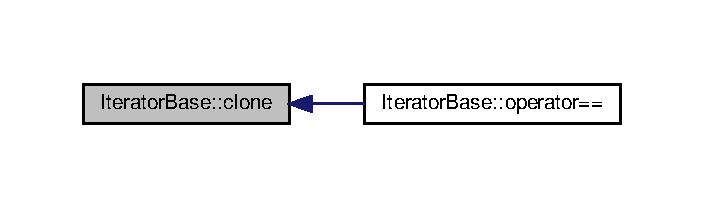
\includegraphics[width=338pt]{class_iterator_base_a541fdf8cc48f31c8ddfdc3f319a37100_icgraph}
\end{center}
\end{figure}
\mbox{\Hypertarget{class_iterator_base_a08430515a17384d098eb62ecce1b64c6}\label{class_iterator_base_a08430515a17384d098eb62ecce1b64c6}} 
\index{Iterator\+Base@{Iterator\+Base}!equal@{equal}}
\index{equal@{equal}!Iterator\+Base@{Iterator\+Base}}
\subsubsection{\texorpdfstring{equal()}{equal()}}
{\footnotesize\ttfamily template$<$typename T$>$ \\
virtual bool \hyperlink{class_iterator_base}{Iterator\+Base}$<$ T $>$\+::equal (\begin{DoxyParamCaption}\item[{const \hyperlink{class_iterator_base}{Iterator\+Base}$<$ T $>$ \&}]{rhs }\end{DoxyParamCaption}) const\hspace{0.3cm}{\ttfamily [protected]}, {\ttfamily [pure virtual]}}



Implémenté dans \hyperlink{class_filtered_iterator_a7118ec2bba2bf138ca771a394a8d72c8}{Filtered\+Iterator$<$ T $>$}, et \hyperlink{class_pool_iterator_adbbef39e72972414b1bbb6d6bb885bb1}{Pool\+Iterator$<$ T $>$}.



Référencé par Iterator\+Base$<$ T $>$\+::operator==().

Voici le graphe des appelants de cette fonction \+:\nopagebreak
\begin{figure}[H]
\begin{center}
\leavevmode
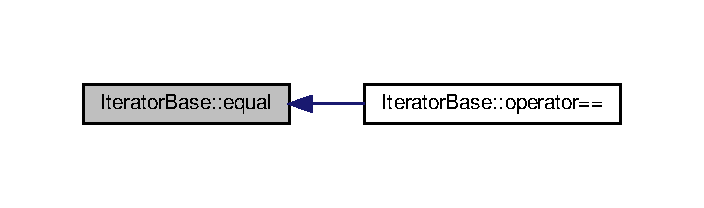
\includegraphics[width=338pt]{class_iterator_base_a08430515a17384d098eb62ecce1b64c6_icgraph}
\end{center}
\end{figure}
\mbox{\Hypertarget{class_iterator_base_a532583e58bce168648bdbdedb3a7d5ab}\label{class_iterator_base_a532583e58bce168648bdbdedb3a7d5ab}} 
\index{Iterator\+Base@{Iterator\+Base}!operator$\ast$@{operator$\ast$}}
\index{operator$\ast$@{operator$\ast$}!Iterator\+Base@{Iterator\+Base}}
\subsubsection{\texorpdfstring{operator$\ast$()}{operator*()}\hspace{0.1cm}{\footnotesize\ttfamily [1/2]}}
{\footnotesize\ttfamily template$<$typename T$>$ \\
virtual T\& \hyperlink{class_iterator_base}{Iterator\+Base}$<$ T $>$\+::operator$\ast$ (\begin{DoxyParamCaption}{ }\end{DoxyParamCaption})\hspace{0.3cm}{\ttfamily [pure virtual]}}



Implémenté dans \hyperlink{class_pool_iterator_a3acdd751b297473d78eedb7422c7a66c}{Pool\+Iterator$<$ T $>$}, et \hyperlink{class_filtered_iterator_ac891b168cd653612ddc7ed7cb4380196}{Filtered\+Iterator$<$ T $>$}.



Référencé par Iterator\+Base$<$ T $>$\+::operator==().

Voici le graphe des appelants de cette fonction \+:\nopagebreak
\begin{figure}[H]
\begin{center}
\leavevmode
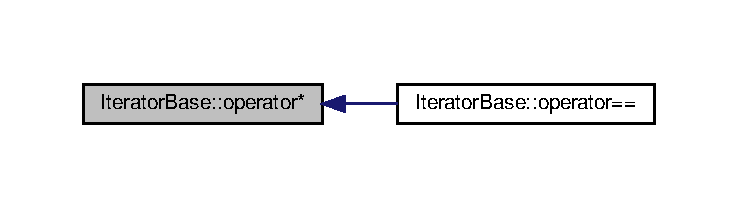
\includegraphics[width=350pt]{class_iterator_base_a532583e58bce168648bdbdedb3a7d5ab_icgraph}
\end{center}
\end{figure}
\mbox{\Hypertarget{class_iterator_base_abc219468b68f2b5471494d04d00f6ec7}\label{class_iterator_base_abc219468b68f2b5471494d04d00f6ec7}} 
\index{Iterator\+Base@{Iterator\+Base}!operator$\ast$@{operator$\ast$}}
\index{operator$\ast$@{operator$\ast$}!Iterator\+Base@{Iterator\+Base}}
\subsubsection{\texorpdfstring{operator$\ast$()}{operator*()}\hspace{0.1cm}{\footnotesize\ttfamily [2/2]}}
{\footnotesize\ttfamily template$<$typename T$>$ \\
virtual const T\& \hyperlink{class_iterator_base}{Iterator\+Base}$<$ T $>$\+::operator$\ast$ (\begin{DoxyParamCaption}{ }\end{DoxyParamCaption}) const\hspace{0.3cm}{\ttfamily [pure virtual]}}



Implémenté dans \hyperlink{class_pool_iterator_ab8a7e0669bfd1cd4335ca726bba77127}{Pool\+Iterator$<$ T $>$}, et \hyperlink{class_filtered_iterator_aab76ce411b72c85c3e6a9007a6c9fd98}{Filtered\+Iterator$<$ T $>$}.

\mbox{\Hypertarget{class_iterator_base_a816f35e9020716d212124a34f1c033fb}\label{class_iterator_base_a816f35e9020716d212124a34f1c033fb}} 
\index{Iterator\+Base@{Iterator\+Base}!operator++@{operator++}}
\index{operator++@{operator++}!Iterator\+Base@{Iterator\+Base}}
\subsubsection{\texorpdfstring{operator++()}{operator++()}}
{\footnotesize\ttfamily template$<$typename T$>$ \\
virtual void \hyperlink{class_iterator_base}{Iterator\+Base}$<$ T $>$\+::operator++ (\begin{DoxyParamCaption}{ }\end{DoxyParamCaption})\hspace{0.3cm}{\ttfamily [pure virtual]}}



Implémenté dans \hyperlink{class_filtered_iterator_ae31347c47637172be3d19dc3be30f5cc}{Filtered\+Iterator$<$ T $>$}, et \hyperlink{class_pool_iterator_a0da86ab88d60973aee45e6a51a929138}{Pool\+Iterator$<$ T $>$}.



Référencé par Iterator\+Base$<$ T $>$\+::operator==().

Voici le graphe des appelants de cette fonction \+:\nopagebreak
\begin{figure}[H]
\begin{center}
\leavevmode
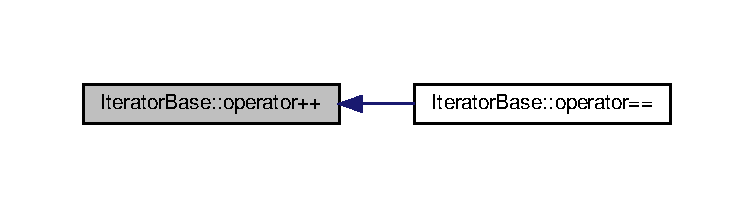
\includegraphics[width=350pt]{class_iterator_base_a816f35e9020716d212124a34f1c033fb_icgraph}
\end{center}
\end{figure}
\mbox{\Hypertarget{class_iterator_base_aa9bf0f75a8bb7e4d416a9b88ccacd9c7}\label{class_iterator_base_aa9bf0f75a8bb7e4d416a9b88ccacd9c7}} 
\index{Iterator\+Base@{Iterator\+Base}!operator-\/-\/@{operator-\/-\/}}
\index{operator-\/-\/@{operator-\/-\/}!Iterator\+Base@{Iterator\+Base}}
\subsubsection{\texorpdfstring{operator-\/-\/()}{operator--()}}
{\footnotesize\ttfamily template$<$typename T$>$ \\
virtual void \hyperlink{class_iterator_base}{Iterator\+Base}$<$ T $>$\+::operator-\/-\/ (\begin{DoxyParamCaption}{ }\end{DoxyParamCaption})\hspace{0.3cm}{\ttfamily [pure virtual]}}



Implémenté dans \hyperlink{class_filtered_iterator_a860a37fdf31e87a96b80cb295e6d34c2}{Filtered\+Iterator$<$ T $>$}, et \hyperlink{class_pool_iterator_aa1f588a47b0c11d6e064e34b129337ae}{Pool\+Iterator$<$ T $>$}.



Référencé par Iterator\+Base$<$ T $>$\+::operator==().

Voici le graphe des appelants de cette fonction \+:\nopagebreak
\begin{figure}[H]
\begin{center}
\leavevmode
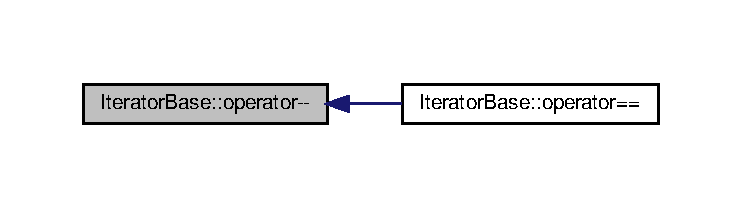
\includegraphics[width=350pt]{class_iterator_base_aa9bf0f75a8bb7e4d416a9b88ccacd9c7_icgraph}
\end{center}
\end{figure}
\mbox{\Hypertarget{class_iterator_base_aad2254f7877e4647f699ceb455e893ff}\label{class_iterator_base_aad2254f7877e4647f699ceb455e893ff}} 
\index{Iterator\+Base@{Iterator\+Base}!operator-\/$>$@{operator-\/$>$}}
\index{operator-\/$>$@{operator-\/$>$}!Iterator\+Base@{Iterator\+Base}}
\subsubsection{\texorpdfstring{operator-\/$>$()}{operator->()}\hspace{0.1cm}{\footnotesize\ttfamily [1/2]}}
{\footnotesize\ttfamily template$<$typename T$>$ \\
virtual T$\ast$ \hyperlink{class_iterator_base}{Iterator\+Base}$<$ T $>$\+::operator-\/$>$ (\begin{DoxyParamCaption}{ }\end{DoxyParamCaption})\hspace{0.3cm}{\ttfamily [pure virtual]}}



Implémenté dans \hyperlink{class_pool_iterator_ae2893041831d8c29f222af7fe184fe09}{Pool\+Iterator$<$ T $>$}, et \hyperlink{class_filtered_iterator_a413726d7cc9a951d0a30eaee6cf36de1}{Filtered\+Iterator$<$ T $>$}.



Référencé par Iterator\+Base$<$ T $>$\+::operator==().

Voici le graphe des appelants de cette fonction \+:\nopagebreak
\begin{figure}[H]
\begin{center}
\leavevmode
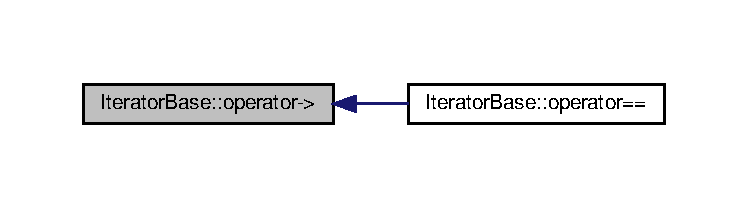
\includegraphics[width=350pt]{class_iterator_base_aad2254f7877e4647f699ceb455e893ff_icgraph}
\end{center}
\end{figure}
\mbox{\Hypertarget{class_iterator_base_a49d96fd63062ca0d7fd813517ad69f03}\label{class_iterator_base_a49d96fd63062ca0d7fd813517ad69f03}} 
\index{Iterator\+Base@{Iterator\+Base}!operator-\/$>$@{operator-\/$>$}}
\index{operator-\/$>$@{operator-\/$>$}!Iterator\+Base@{Iterator\+Base}}
\subsubsection{\texorpdfstring{operator-\/$>$()}{operator->()}\hspace{0.1cm}{\footnotesize\ttfamily [2/2]}}
{\footnotesize\ttfamily template$<$typename T$>$ \\
virtual const T$\ast$ \hyperlink{class_iterator_base}{Iterator\+Base}$<$ T $>$\+::operator-\/$>$ (\begin{DoxyParamCaption}{ }\end{DoxyParamCaption}) const\hspace{0.3cm}{\ttfamily [pure virtual]}}



Implémenté dans \hyperlink{class_pool_iterator_a228d6ee24cd015a7312fa9f76244994c}{Pool\+Iterator$<$ T $>$}, et \hyperlink{class_filtered_iterator_a75ea4ec86c45f496c1515e8e9832cd0f}{Filtered\+Iterator$<$ T $>$}.

\mbox{\Hypertarget{class_iterator_base_a7475728422cb73f91d1c4cb4c3d07499}\label{class_iterator_base_a7475728422cb73f91d1c4cb4c3d07499}} 
\index{Iterator\+Base@{Iterator\+Base}!operator==@{operator==}}
\index{operator==@{operator==}!Iterator\+Base@{Iterator\+Base}}
\subsubsection{\texorpdfstring{operator==()}{operator==()}}
{\footnotesize\ttfamily template$<$typename T$>$ \\
bool \hyperlink{class_iterator_base}{Iterator\+Base}$<$ T $>$\+::operator== (\begin{DoxyParamCaption}\item[{const \hyperlink{class_iterator_base}{Iterator\+Base}$<$ T $>$ \&}]{rhs }\end{DoxyParamCaption}) const\hspace{0.3cm}{\ttfamily [inline]}}



Références Iterator\+Base$<$ T $>$\+::clone(), Iterator\+Base$<$ T $>$\+::equal(), Iterator\+Base$<$ T $>$\+::operator$\ast$(), Iterator\+Base$<$ T $>$\+::operator++(), Iterator\+Base$<$ T $>$\+::operator-\/-\/(), et Iterator\+Base$<$ T $>$\+::operator-\/$>$().

Voici le graphe d\textquotesingle{}appel pour cette fonction \+:\nopagebreak
\begin{figure}[H]
\begin{center}
\leavevmode
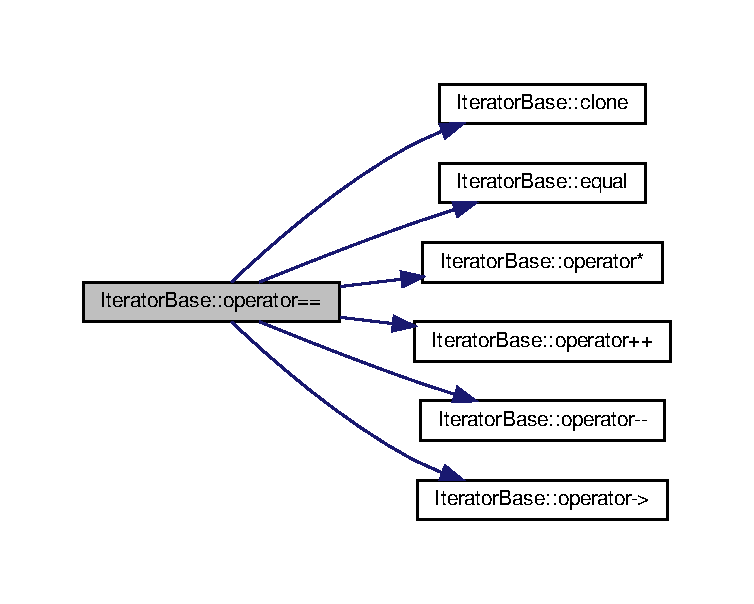
\includegraphics[width=350pt]{class_iterator_base_a7475728422cb73f91d1c4cb4c3d07499_cgraph}
\end{center}
\end{figure}


La documentation de cette classe a été générée à partir du fichier suivant \+:\begin{DoxyCompactItemize}
\item 
src/\hyperlink{_collection_iterator_8hpp}{Collection\+Iterator.\+hpp}\end{DoxyCompactItemize}

\hypertarget{class_pool_iterator}{}\section{Référence du modèle de la classe Pool\+Iterator$<$ T $>$}
\label{class_pool_iterator}\index{Pool\+Iterator$<$ T $>$@{Pool\+Iterator$<$ T $>$}}


{\ttfamily \#include $<$Collection\+Pool.\+hpp$>$}



Graphe d\textquotesingle{}héritage de Pool\+Iterator$<$ T $>$\+:\nopagebreak
\begin{figure}[H]
\begin{center}
\leavevmode
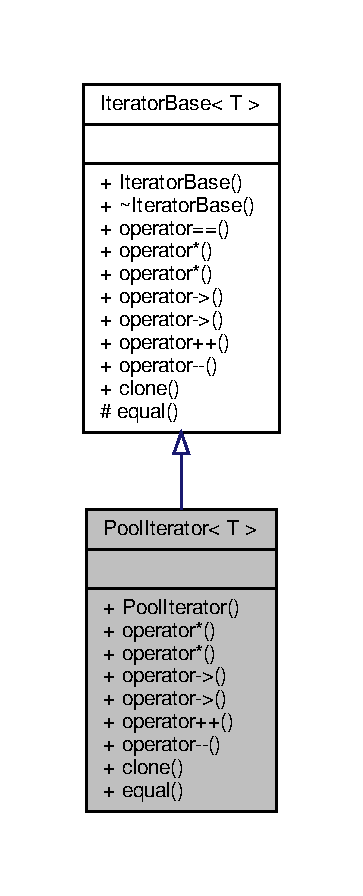
\includegraphics[width=174pt]{class_pool_iterator__inherit__graph}
\end{center}
\end{figure}


Graphe de collaboration de Pool\+Iterator$<$ T $>$\+:\nopagebreak
\begin{figure}[H]
\begin{center}
\leavevmode
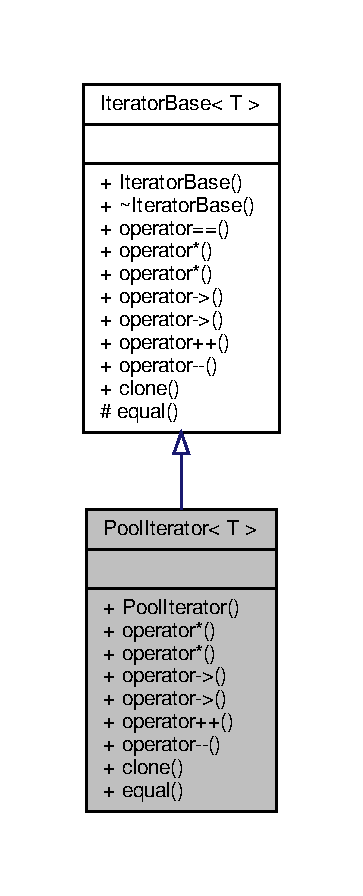
\includegraphics[width=174pt]{class_pool_iterator__coll__graph}
\end{center}
\end{figure}
\subsection*{Fonctions membres publiques}
\begin{DoxyCompactItemize}
\item 
\hyperlink{class_pool_iterator_a5c4bd22679d557a14326b018850874bb}{Pool\+Iterator} (T $\ast$ptr)
\item 
T \& \hyperlink{class_pool_iterator_a3acdd751b297473d78eedb7422c7a66c}{operator$\ast$} () override
\item 
const T \& \hyperlink{class_pool_iterator_ab8a7e0669bfd1cd4335ca726bba77127}{operator$\ast$} () const override
\item 
T $\ast$ \hyperlink{class_pool_iterator_ae2893041831d8c29f222af7fe184fe09}{operator-\/$>$} () override
\item 
const T $\ast$ \hyperlink{class_pool_iterator_a228d6ee24cd015a7312fa9f76244994c}{operator-\/$>$} () const override
\item 
void \hyperlink{class_pool_iterator_a0da86ab88d60973aee45e6a51a929138}{operator++} () override
\item 
void \hyperlink{class_pool_iterator_aa1f588a47b0c11d6e064e34b129337ae}{operator-\/-\/} () override
\item 
\hyperlink{class_iterator_base}{Iterator\+Base}$<$ T $>$ $\ast$ \hyperlink{class_pool_iterator_ae39cdb4bbb84e88cf0d9009e7bdae586}{clone} () const override
\item 
bool \hyperlink{class_pool_iterator_adbbef39e72972414b1bbb6d6bb885bb1}{equal} (const \hyperlink{class_iterator_base}{Iterator\+Base}$<$ T $>$ \&rhs) const override
\end{DoxyCompactItemize}
\subsection*{Membres hérités additionnels}


\subsection{Documentation des constructeurs et destructeur}
\mbox{\Hypertarget{class_pool_iterator_a5c4bd22679d557a14326b018850874bb}\label{class_pool_iterator_a5c4bd22679d557a14326b018850874bb}} 
\index{Pool\+Iterator@{Pool\+Iterator}!Pool\+Iterator@{Pool\+Iterator}}
\index{Pool\+Iterator@{Pool\+Iterator}!Pool\+Iterator@{Pool\+Iterator}}
\subsubsection{\texorpdfstring{Pool\+Iterator()}{PoolIterator()}}
{\footnotesize\ttfamily template$<$typename T $>$ \\
\hyperlink{class_pool_iterator}{Pool\+Iterator}$<$ T $>$\+::\hyperlink{class_pool_iterator}{Pool\+Iterator} (\begin{DoxyParamCaption}\item[{T $\ast$}]{ptr }\end{DoxyParamCaption})\hspace{0.3cm}{\ttfamily [inline]}, {\ttfamily [explicit]}}



\subsection{Documentation des fonctions membres}
\mbox{\Hypertarget{class_pool_iterator_ae39cdb4bbb84e88cf0d9009e7bdae586}\label{class_pool_iterator_ae39cdb4bbb84e88cf0d9009e7bdae586}} 
\index{Pool\+Iterator@{Pool\+Iterator}!clone@{clone}}
\index{clone@{clone}!Pool\+Iterator@{Pool\+Iterator}}
\subsubsection{\texorpdfstring{clone()}{clone()}}
{\footnotesize\ttfamily template$<$typename T $>$ \\
\hyperlink{class_iterator_base}{Iterator\+Base}$<$T$>$$\ast$ \hyperlink{class_pool_iterator}{Pool\+Iterator}$<$ T $>$\+::clone (\begin{DoxyParamCaption}{ }\end{DoxyParamCaption}) const\hspace{0.3cm}{\ttfamily [inline]}, {\ttfamily [override]}, {\ttfamily [virtual]}}



Implémente \hyperlink{class_iterator_base_a541fdf8cc48f31c8ddfdc3f319a37100}{Iterator\+Base$<$ T $>$}.

\mbox{\Hypertarget{class_pool_iterator_adbbef39e72972414b1bbb6d6bb885bb1}\label{class_pool_iterator_adbbef39e72972414b1bbb6d6bb885bb1}} 
\index{Pool\+Iterator@{Pool\+Iterator}!equal@{equal}}
\index{equal@{equal}!Pool\+Iterator@{Pool\+Iterator}}
\subsubsection{\texorpdfstring{equal()}{equal()}}
{\footnotesize\ttfamily template$<$typename T $>$ \\
bool \hyperlink{class_pool_iterator}{Pool\+Iterator}$<$ T $>$\+::equal (\begin{DoxyParamCaption}\item[{const \hyperlink{class_iterator_base}{Iterator\+Base}$<$ T $>$ \&}]{rhs }\end{DoxyParamCaption}) const\hspace{0.3cm}{\ttfamily [inline]}, {\ttfamily [override]}, {\ttfamily [virtual]}}



Implémente \hyperlink{class_iterator_base_a08430515a17384d098eb62ecce1b64c6}{Iterator\+Base$<$ T $>$}.

\mbox{\Hypertarget{class_pool_iterator_a3acdd751b297473d78eedb7422c7a66c}\label{class_pool_iterator_a3acdd751b297473d78eedb7422c7a66c}} 
\index{Pool\+Iterator@{Pool\+Iterator}!operator$\ast$@{operator$\ast$}}
\index{operator$\ast$@{operator$\ast$}!Pool\+Iterator@{Pool\+Iterator}}
\subsubsection{\texorpdfstring{operator$\ast$()}{operator*()}\hspace{0.1cm}{\footnotesize\ttfamily [1/2]}}
{\footnotesize\ttfamily template$<$typename T $>$ \\
T\& \hyperlink{class_pool_iterator}{Pool\+Iterator}$<$ T $>$\+::operator$\ast$ (\begin{DoxyParamCaption}{ }\end{DoxyParamCaption})\hspace{0.3cm}{\ttfamily [inline]}, {\ttfamily [override]}, {\ttfamily [virtual]}}



Implémente \hyperlink{class_iterator_base_a532583e58bce168648bdbdedb3a7d5ab}{Iterator\+Base$<$ T $>$}.

\mbox{\Hypertarget{class_pool_iterator_ab8a7e0669bfd1cd4335ca726bba77127}\label{class_pool_iterator_ab8a7e0669bfd1cd4335ca726bba77127}} 
\index{Pool\+Iterator@{Pool\+Iterator}!operator$\ast$@{operator$\ast$}}
\index{operator$\ast$@{operator$\ast$}!Pool\+Iterator@{Pool\+Iterator}}
\subsubsection{\texorpdfstring{operator$\ast$()}{operator*()}\hspace{0.1cm}{\footnotesize\ttfamily [2/2]}}
{\footnotesize\ttfamily template$<$typename T $>$ \\
const T\& \hyperlink{class_pool_iterator}{Pool\+Iterator}$<$ T $>$\+::operator$\ast$ (\begin{DoxyParamCaption}{ }\end{DoxyParamCaption}) const\hspace{0.3cm}{\ttfamily [inline]}, {\ttfamily [override]}, {\ttfamily [virtual]}}



Implémente \hyperlink{class_iterator_base_abc219468b68f2b5471494d04d00f6ec7}{Iterator\+Base$<$ T $>$}.

\mbox{\Hypertarget{class_pool_iterator_a0da86ab88d60973aee45e6a51a929138}\label{class_pool_iterator_a0da86ab88d60973aee45e6a51a929138}} 
\index{Pool\+Iterator@{Pool\+Iterator}!operator++@{operator++}}
\index{operator++@{operator++}!Pool\+Iterator@{Pool\+Iterator}}
\subsubsection{\texorpdfstring{operator++()}{operator++()}}
{\footnotesize\ttfamily template$<$typename T $>$ \\
void \hyperlink{class_pool_iterator}{Pool\+Iterator}$<$ T $>$\+::operator++ (\begin{DoxyParamCaption}{ }\end{DoxyParamCaption})\hspace{0.3cm}{\ttfamily [inline]}, {\ttfamily [override]}, {\ttfamily [virtual]}}



Implémente \hyperlink{class_iterator_base_a816f35e9020716d212124a34f1c033fb}{Iterator\+Base$<$ T $>$}.

\mbox{\Hypertarget{class_pool_iterator_aa1f588a47b0c11d6e064e34b129337ae}\label{class_pool_iterator_aa1f588a47b0c11d6e064e34b129337ae}} 
\index{Pool\+Iterator@{Pool\+Iterator}!operator-\/-\/@{operator-\/-\/}}
\index{operator-\/-\/@{operator-\/-\/}!Pool\+Iterator@{Pool\+Iterator}}
\subsubsection{\texorpdfstring{operator-\/-\/()}{operator--()}}
{\footnotesize\ttfamily template$<$typename T $>$ \\
void \hyperlink{class_pool_iterator}{Pool\+Iterator}$<$ T $>$\+::operator-\/-\/ (\begin{DoxyParamCaption}{ }\end{DoxyParamCaption})\hspace{0.3cm}{\ttfamily [inline]}, {\ttfamily [override]}, {\ttfamily [virtual]}}



Implémente \hyperlink{class_iterator_base_aa9bf0f75a8bb7e4d416a9b88ccacd9c7}{Iterator\+Base$<$ T $>$}.

\mbox{\Hypertarget{class_pool_iterator_ae2893041831d8c29f222af7fe184fe09}\label{class_pool_iterator_ae2893041831d8c29f222af7fe184fe09}} 
\index{Pool\+Iterator@{Pool\+Iterator}!operator-\/$>$@{operator-\/$>$}}
\index{operator-\/$>$@{operator-\/$>$}!Pool\+Iterator@{Pool\+Iterator}}
\subsubsection{\texorpdfstring{operator-\/$>$()}{operator->()}\hspace{0.1cm}{\footnotesize\ttfamily [1/2]}}
{\footnotesize\ttfamily template$<$typename T $>$ \\
T$\ast$ \hyperlink{class_pool_iterator}{Pool\+Iterator}$<$ T $>$\+::operator-\/$>$ (\begin{DoxyParamCaption}{ }\end{DoxyParamCaption})\hspace{0.3cm}{\ttfamily [inline]}, {\ttfamily [override]}, {\ttfamily [virtual]}}



Implémente \hyperlink{class_iterator_base_aad2254f7877e4647f699ceb455e893ff}{Iterator\+Base$<$ T $>$}.

\mbox{\Hypertarget{class_pool_iterator_a228d6ee24cd015a7312fa9f76244994c}\label{class_pool_iterator_a228d6ee24cd015a7312fa9f76244994c}} 
\index{Pool\+Iterator@{Pool\+Iterator}!operator-\/$>$@{operator-\/$>$}}
\index{operator-\/$>$@{operator-\/$>$}!Pool\+Iterator@{Pool\+Iterator}}
\subsubsection{\texorpdfstring{operator-\/$>$()}{operator->()}\hspace{0.1cm}{\footnotesize\ttfamily [2/2]}}
{\footnotesize\ttfamily template$<$typename T $>$ \\
const T$\ast$ \hyperlink{class_pool_iterator}{Pool\+Iterator}$<$ T $>$\+::operator-\/$>$ (\begin{DoxyParamCaption}{ }\end{DoxyParamCaption}) const\hspace{0.3cm}{\ttfamily [inline]}, {\ttfamily [override]}, {\ttfamily [virtual]}}



Implémente \hyperlink{class_iterator_base_a49d96fd63062ca0d7fd813517ad69f03}{Iterator\+Base$<$ T $>$}.



La documentation de cette classe a été générée à partir du fichier suivant \+:\begin{DoxyCompactItemize}
\item 
src/\hyperlink{_collection_pool_8hpp}{Collection\+Pool.\+hpp}\end{DoxyCompactItemize}

\chapter{Documentation des fichiers}
\hypertarget{_collection_8hpp}{}\section{Référence du fichier src/\+Collection.hpp}
\label{_collection_8hpp}\index{src/\+Collection.\+hpp@{src/\+Collection.\+hpp}}
{\ttfamily \#include \char`\"{}Collection\+Iterator.\+hpp\char`\"{}}\newline
{\ttfamily \#include $<$iterator$>$}\newline
Graphe des dépendances par inclusion de Collection.\+hpp\+:\nopagebreak
\begin{figure}[H]
\begin{center}
\leavevmode
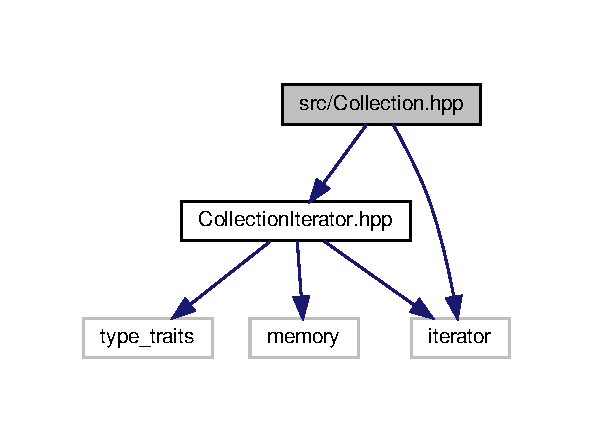
\includegraphics[width=285pt]{_collection_8hpp__incl}
\end{center}
\end{figure}
Ce graphe montre quels fichiers incluent directement ou indirectement ce fichier \+:\nopagebreak
\begin{figure}[H]
\begin{center}
\leavevmode
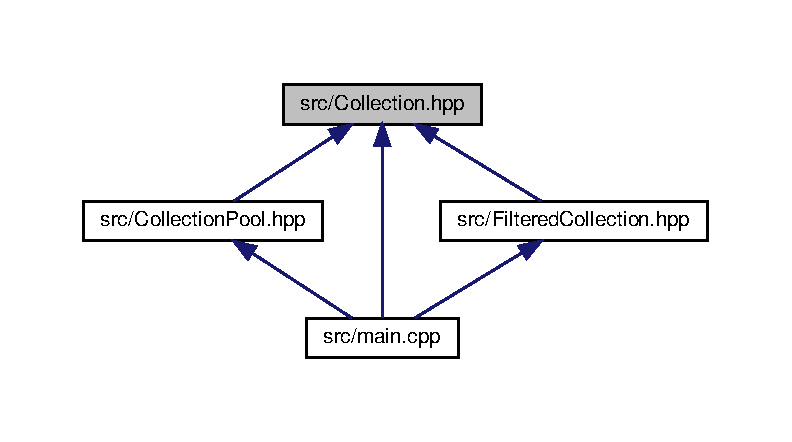
\includegraphics[width=350pt]{_collection_8hpp__dep__incl}
\end{center}
\end{figure}
\subsection*{Classes}
\begin{DoxyCompactItemize}
\item 
class \hyperlink{class_collection}{Collection$<$ T $>$}
\end{DoxyCompactItemize}

\hypertarget{_collection_iterator_8hpp}{}\section{Référence du fichier src/\+Collection\+Iterator.hpp}
\label{_collection_iterator_8hpp}\index{src/\+Collection\+Iterator.\+hpp@{src/\+Collection\+Iterator.\+hpp}}
{\ttfamily \#include $<$type\+\_\+traits$>$}\newline
{\ttfamily \#include $<$iterator$>$}\newline
{\ttfamily \#include $<$memory$>$}\newline
Graphe des dépendances par inclusion de Collection\+Iterator.\+hpp\+:\nopagebreak
\begin{figure}[H]
\begin{center}
\leavevmode
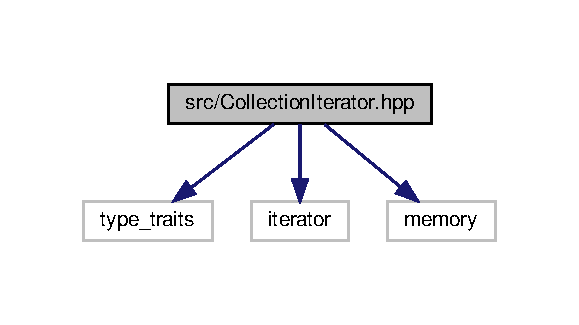
\includegraphics[width=278pt]{_collection_iterator_8hpp__incl}
\end{center}
\end{figure}
Ce graphe montre quels fichiers incluent directement ou indirectement ce fichier \+:\nopagebreak
\begin{figure}[H]
\begin{center}
\leavevmode
\includegraphics[width=350pt]{_collection_iterator_8hpp__dep__incl}
\end{center}
\end{figure}
\subsection*{Classes}
\begin{DoxyCompactItemize}
\item 
class \hyperlink{class_iterator_base}{Iterator\+Base$<$ T $>$}
\item 
class \hyperlink{class_collection_iterator}{Collection\+Iterator$<$ T $>$}
\end{DoxyCompactItemize}

\hypertarget{_collection_pool_8hpp}{}\section{Référence du fichier src/\+Collection\+Pool.hpp}
\label{_collection_pool_8hpp}\index{src/\+Collection\+Pool.\+hpp@{src/\+Collection\+Pool.\+hpp}}
{\ttfamily \#include \char`\"{}Collection.\+hpp\char`\"{}}\newline
{\ttfamily \#include \char`\"{}Collection\+Iterator.\+hpp\char`\"{}}\newline
{\ttfamily \#include $<$vector$>$}\newline
{\ttfamily \#include $<$iterator$>$}\newline
Graphe des dépendances par inclusion de Collection\+Pool.\+hpp\+:\nopagebreak
\begin{figure}[H]
\begin{center}
\leavevmode
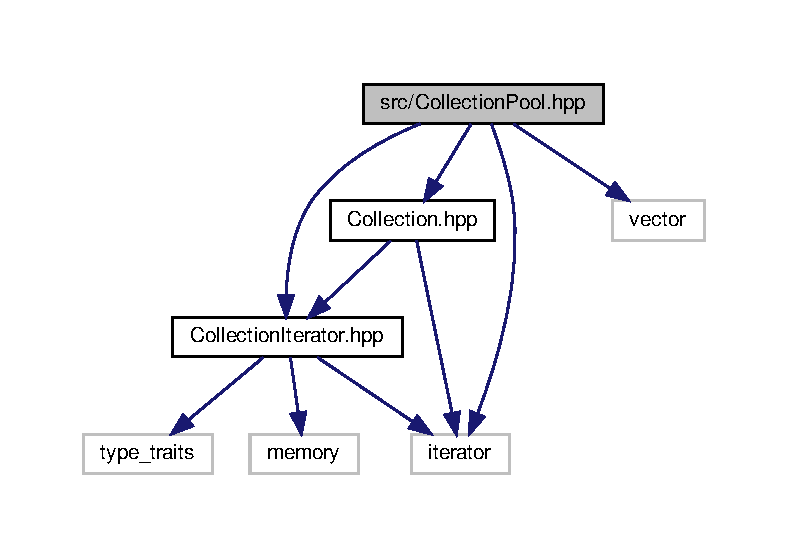
\includegraphics[width=350pt]{_collection_pool_8hpp__incl}
\end{center}
\end{figure}
Ce graphe montre quels fichiers incluent directement ou indirectement ce fichier \+:\nopagebreak
\begin{figure}[H]
\begin{center}
\leavevmode
\includegraphics[width=195pt]{_collection_pool_8hpp__dep__incl}
\end{center}
\end{figure}
\subsection*{Classes}
\begin{DoxyCompactItemize}
\item 
class \hyperlink{class_pool_iterator}{Pool\+Iterator$<$ T $>$}
\item 
class \hyperlink{class_collection_pool}{Collection\+Pool$<$ T $>$}
\item 
class \hyperlink{class_pool_iterator}{Pool\+Iterator$<$ T $>$}
\end{DoxyCompactItemize}

\hypertarget{_file_dialog_8hpp}{}\section{Référence du fichier src/\+File\+Dialog.hpp}
\label{_file_dialog_8hpp}\index{src/\+File\+Dialog.\+hpp@{src/\+File\+Dialog.\+hpp}}
{\ttfamily \#include $<$experimental/filesystem$>$}\newline
{\ttfamily \#include $<$string$>$}\newline
Graphe des dépendances par inclusion de File\+Dialog.\+hpp\+:\nopagebreak
\begin{figure}[H]
\begin{center}
\leavevmode
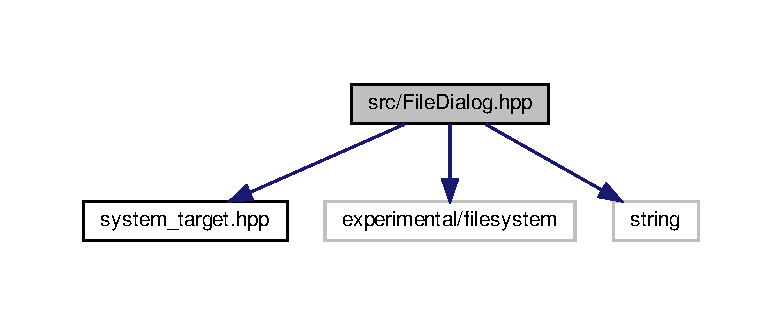
\includegraphics[width=260pt]{_file_dialog_8hpp__incl}
\end{center}
\end{figure}
Ce graphe montre quels fichiers incluent directement ou indirectement ce fichier \+:\nopagebreak
\begin{figure}[H]
\begin{center}
\leavevmode
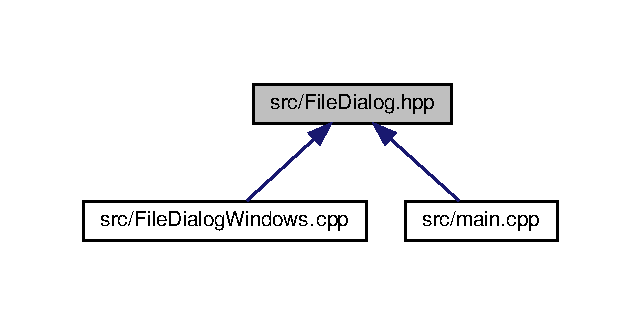
\includegraphics[width=308pt]{_file_dialog_8hpp__dep__incl}
\end{center}
\end{figure}
\subsection*{Classes}
\begin{DoxyCompactItemize}
\item 
struct \hyperlink{structfile__filter}{file\+\_\+filter}
\end{DoxyCompactItemize}
\subsection*{Fonctions}
\begin{DoxyCompactItemize}
\item 
std\+::experimental\+::filesystem\+::path \hyperlink{_file_dialog_8hpp_aff1c082fbf12dfb78f3668367291cfa0}{get\+Open\+File\+Name} (const std\+::string \&title=\char`\"{}Open a file\char`\"{}, const \hyperlink{structfile__filter}{file\+\_\+filter} \&filter=\{\char`\"{}All files\char`\"{}, \char`\"{}$\ast$\char`\"{}\}, const std\+::experimental\+::filesystem\+::path \&initial\+Dir=\char`\"{}\char`\"{})
\begin{DoxyCompactList}\small\item\em Ouvre une boîte de dialogue qui demande un fichier à ouvrir. \end{DoxyCompactList}\item 
std\+::experimental\+::filesystem\+::path \hyperlink{_file_dialog_8hpp_ad8785c85930dceac9ba4610e852cf0c1}{get\+Save\+File\+Name} (const std\+::string \&title=\char`\"{}Save file as\char`\"{}, const \hyperlink{structfile__filter}{file\+\_\+filter} \&filter=\{\char`\"{}All files\char`\"{}, \char`\"{}$\ast$\char`\"{}\}, const std\+::string \&initial\+Dir=\char`\"{}\char`\"{})
\begin{DoxyCompactList}\small\item\em Ouvre une boîte de dialogue qui demande un nom de sauvegarde pour un fichier. \end{DoxyCompactList}\item 
std\+::experimental\+::filesystem\+::path \hyperlink{_file_dialog_8hpp_a9fbbe1b6f277e71376b51951e9eee619}{browse\+Folder} (const std\+::string \&title=\char`\"{}Select a directory\char`\"{}, const std\+::string \&initial\+Dir=\char`\"{}\char`\"{})
\begin{DoxyCompactList}\small\item\em Ouvre une boîte de dialogue qui demande un répertoire à ouvrir. \end{DoxyCompactList}\end{DoxyCompactItemize}


\subsection{Documentation des fonctions}
\mbox{\Hypertarget{_file_dialog_8hpp_a9fbbe1b6f277e71376b51951e9eee619}\label{_file_dialog_8hpp_a9fbbe1b6f277e71376b51951e9eee619}} 
\index{File\+Dialog.\+hpp@{File\+Dialog.\+hpp}!browse\+Folder@{browse\+Folder}}
\index{browse\+Folder@{browse\+Folder}!File\+Dialog.\+hpp@{File\+Dialog.\+hpp}}
\subsubsection{\texorpdfstring{browse\+Folder()}{browseFolder()}}
{\footnotesize\ttfamily std\+::experimental\+::filesystem\+::path browse\+Folder (\begin{DoxyParamCaption}\item[{const std\+::string \&}]{title = {\ttfamily \char`\"{}Select~a~directory\char`\"{}},  }\item[{const std\+::string \&}]{initial\+Dir = {\ttfamily \char`\"{}\char`\"{}} }\end{DoxyParamCaption})}



Ouvre une boîte de dialogue qui demande un répertoire à ouvrir. 


\begin{DoxyParams}{Paramètres}
{\em title} & titre de la boîte de dialogue \\
\hline
{\em initial\+Dir} & Dossier dans lequel se trouvera la boîte de dialogue à l\textquotesingle{}ouverture \\
\hline
\end{DoxyParams}
\begin{DoxyReturn}{Renvoie}
chemin vers le répertoire sélectionné 
\end{DoxyReturn}
\mbox{\Hypertarget{_file_dialog_8hpp_aff1c082fbf12dfb78f3668367291cfa0}\label{_file_dialog_8hpp_aff1c082fbf12dfb78f3668367291cfa0}} 
\index{File\+Dialog.\+hpp@{File\+Dialog.\+hpp}!get\+Open\+File\+Name@{get\+Open\+File\+Name}}
\index{get\+Open\+File\+Name@{get\+Open\+File\+Name}!File\+Dialog.\+hpp@{File\+Dialog.\+hpp}}
\subsubsection{\texorpdfstring{get\+Open\+File\+Name()}{getOpenFileName()}}
{\footnotesize\ttfamily std\+::experimental\+::filesystem\+::path get\+Open\+File\+Name (\begin{DoxyParamCaption}\item[{const std\+::string \&}]{title = {\ttfamily \char`\"{}Open~a~file\char`\"{}},  }\item[{const \hyperlink{structfile__filter}{file\+\_\+filter} \&}]{filter = {\ttfamily \{\char`\"{}All~files\char`\"{},~\char`\"{}$\ast$\char`\"{}\}},  }\item[{const std\+::experimental\+::filesystem\+::path \&}]{initial\+Dir = {\ttfamily \char`\"{}\char`\"{}} }\end{DoxyParamCaption})}



Ouvre une boîte de dialogue qui demande un fichier à ouvrir. 


\begin{DoxyParams}{Paramètres}
{\em title} & titre de la boîte de dialogue \\
\hline
{\em filter} & filtre sur les fichiers à ouvrir \\
\hline
{\em initial\+Dir} & Dossier dans lequel se trouvera la boîte de dialogue à l\textquotesingle{}ouverture \\
\hline
\end{DoxyParams}
\begin{DoxyReturn}{Renvoie}
chemin vers le fichier sélectionné 
\end{DoxyReturn}


Référencé par main().

Voici le graphe des appelants de cette fonction \+:\nopagebreak
\begin{figure}[H]
\begin{center}
\leavevmode
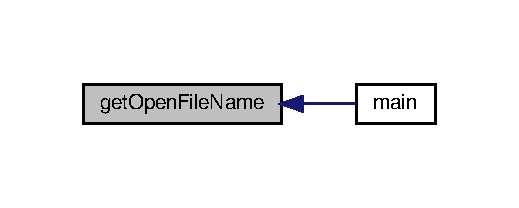
\includegraphics[width=249pt]{_file_dialog_8hpp_aff1c082fbf12dfb78f3668367291cfa0_icgraph}
\end{center}
\end{figure}
\mbox{\Hypertarget{_file_dialog_8hpp_ad8785c85930dceac9ba4610e852cf0c1}\label{_file_dialog_8hpp_ad8785c85930dceac9ba4610e852cf0c1}} 
\index{File\+Dialog.\+hpp@{File\+Dialog.\+hpp}!get\+Save\+File\+Name@{get\+Save\+File\+Name}}
\index{get\+Save\+File\+Name@{get\+Save\+File\+Name}!File\+Dialog.\+hpp@{File\+Dialog.\+hpp}}
\subsubsection{\texorpdfstring{get\+Save\+File\+Name()}{getSaveFileName()}}
{\footnotesize\ttfamily std\+::experimental\+::filesystem\+::path get\+Save\+File\+Name (\begin{DoxyParamCaption}\item[{const std\+::string \&}]{title = {\ttfamily \char`\"{}Save~file~as\char`\"{}},  }\item[{const \hyperlink{structfile__filter}{file\+\_\+filter} \&}]{filter = {\ttfamily \{\char`\"{}All~files\char`\"{},~\char`\"{}$\ast$\char`\"{}\}},  }\item[{const std\+::string \&}]{initial\+Dir = {\ttfamily \char`\"{}\char`\"{}} }\end{DoxyParamCaption})}



Ouvre une boîte de dialogue qui demande un nom de sauvegarde pour un fichier. 


\begin{DoxyParams}{Paramètres}
{\em title} & titre de la boîte de dialogue \\
\hline
{\em filter} & filtre sur les fichiers à ouvrir \\
\hline
{\em initial\+Dir} & Dossier dans lequel se trouvera la boîte de dialogue à l\textquotesingle{}ouverture \\
\hline
\end{DoxyParams}
\begin{DoxyReturn}{Renvoie}
chemin de sauvegarde du fichier 
\end{DoxyReturn}

\hypertarget{_file_dialog_linux_8cpp}{}\section{Référence du fichier src/\+File\+Dialog\+Linux.cpp}
\label{_file_dialog_linux_8cpp}\index{src/\+File\+Dialog\+Linux.\+cpp@{src/\+File\+Dialog\+Linux.\+cpp}}

\hypertarget{_file_dialog_windows_8cpp}{}\section{Référence du fichier src/\+File\+Dialog\+Windows.cpp}
\label{_file_dialog_windows_8cpp}\index{src/\+File\+Dialog\+Windows.\+cpp@{src/\+File\+Dialog\+Windows.\+cpp}}
{\ttfamily \#include \char`\"{}File\+Dialog.\+hpp\char`\"{}}\newline
Graphe des dépendances par inclusion de File\+Dialog\+Windows.\+cpp\+:\nopagebreak
\begin{figure}[H]
\begin{center}
\leavevmode
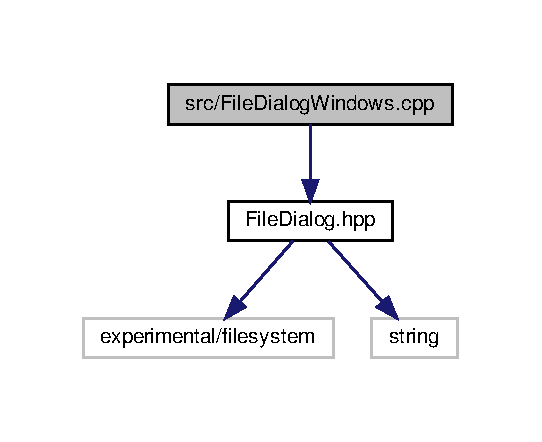
\includegraphics[width=350pt]{_file_dialog_windows_8cpp__incl}
\end{center}
\end{figure}

\hypertarget{_filtered_collection_8hpp}{}\section{Référence du fichier src/\+Filtered\+Collection.hpp}
\label{_filtered_collection_8hpp}\index{src/\+Filtered\+Collection.\+hpp@{src/\+Filtered\+Collection.\+hpp}}
{\ttfamily \#include \char`\"{}Collection.\+hpp\char`\"{}}\newline
{\ttfamily \#include $<$vector$>$}\newline
{\ttfamily \#include $<$functional$>$}\newline
Graphe des dépendances par inclusion de Filtered\+Collection.\+hpp\+:\nopagebreak
\begin{figure}[H]
\begin{center}
\leavevmode
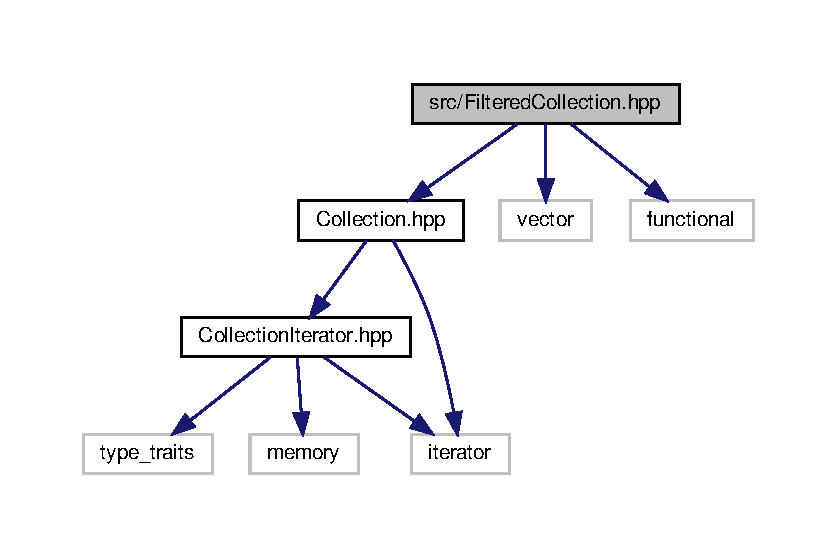
\includegraphics[width=350pt]{_filtered_collection_8hpp__incl}
\end{center}
\end{figure}
Ce graphe montre quels fichiers incluent directement ou indirectement ce fichier \+:\nopagebreak
\begin{figure}[H]
\begin{center}
\leavevmode
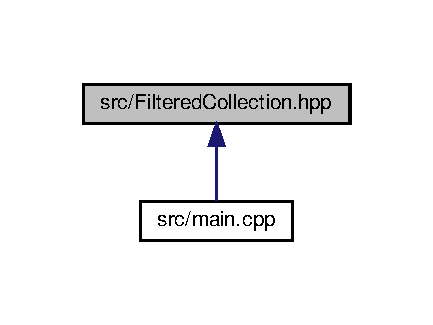
\includegraphics[width=208pt]{_filtered_collection_8hpp__dep__incl}
\end{center}
\end{figure}
\subsection*{Classes}
\begin{DoxyCompactItemize}
\item 
class \hyperlink{class_filtered_iterator}{Filtered\+Iterator$<$ T $>$}
\item 
class \hyperlink{class_filtered_collection}{Filtered\+Collection$<$ T $>$}
\item 
class \hyperlink{class_filtered_iterator}{Filtered\+Iterator$<$ T $>$}
\end{DoxyCompactItemize}

\hypertarget{_image_8hpp}{}\section{Référence du fichier src/\+Image.hpp}
\label{_image_8hpp}\index{src/\+Image.\+hpp@{src/\+Image.\+hpp}}
{\ttfamily \#include \char`\"{}Tag\+List.\+hpp\char`\"{}}\newline
{\ttfamily \#include $<$experimental/filesystem$>$}\newline
{\ttfamily \#include $<$memory$>$}\newline
Graphe des dépendances par inclusion de Image.\+hpp\+:\nopagebreak
\begin{figure}[H]
\begin{center}
\leavevmode
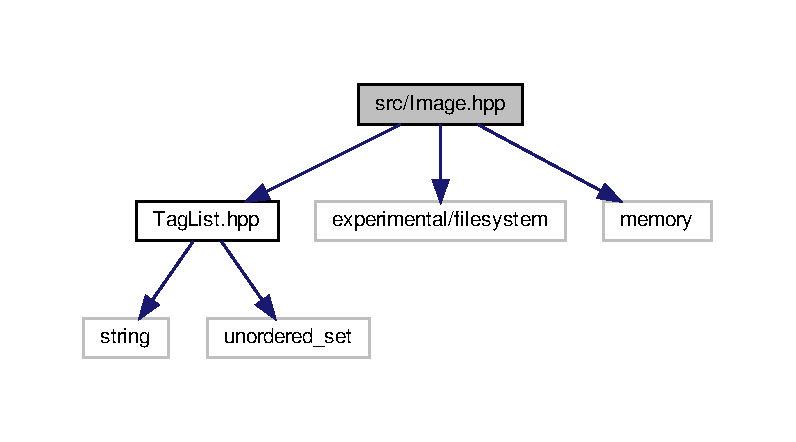
\includegraphics[width=350pt]{_image_8hpp__incl}
\end{center}
\end{figure}
Ce graphe montre quels fichiers incluent directement ou indirectement ce fichier \+:\nopagebreak
\begin{figure}[H]
\begin{center}
\leavevmode
\includegraphics[width=159pt]{_image_8hpp__dep__incl}
\end{center}
\end{figure}
\subsection*{Classes}
\begin{DoxyCompactItemize}
\item 
class \hyperlink{class_image}{Image$<$ img\+\_\+t $>$}
\end{DoxyCompactItemize}

\hypertarget{main_8cpp}{}\section{Référence du fichier src/main.cpp}
\label{main_8cpp}\index{src/main.\+cpp@{src/main.\+cpp}}
{\ttfamily \#include \char`\"{}Collection\+Iterator.\+hpp\char`\"{}}\newline
{\ttfamily \#include \char`\"{}File\+Dialog.\+hpp\char`\"{}}\newline
{\ttfamily \#include \char`\"{}Filtered\+Collection.\+hpp\char`\"{}}\newline
{\ttfamily \#include \char`\"{}Collection.\+hpp\char`\"{}}\newline
{\ttfamily \#include \char`\"{}Collection\+Pool.\+hpp\char`\"{}}\newline
{\ttfamily \#include \char`\"{}Image.\+hpp\char`\"{}}\newline
{\ttfamily \#include $<$iostream$>$}\newline
{\ttfamily \#include $<$experimental/filesystem$>$}\newline
Graphe des dépendances par inclusion de main.\+cpp\+:\nopagebreak
\begin{figure}[H]
\begin{center}
\leavevmode
\includegraphics[width=350pt]{main_8cpp__incl}
\end{center}
\end{figure}
\subsection*{Fonctions}
\begin{DoxyCompactItemize}
\item 
bool \hyperlink{main_8cpp_a7e2279174c7277e845bae3e68568d1b4}{is\+Pair} (const int \&i)
\item 
int \hyperlink{main_8cpp_ae66f6b31b5ad750f1fe042a706a4e3d4}{main} ()
\end{DoxyCompactItemize}


\subsection{Documentation des fonctions}
\mbox{\Hypertarget{main_8cpp_a7e2279174c7277e845bae3e68568d1b4}\label{main_8cpp_a7e2279174c7277e845bae3e68568d1b4}} 
\index{main.\+cpp@{main.\+cpp}!is\+Pair@{is\+Pair}}
\index{is\+Pair@{is\+Pair}!main.\+cpp@{main.\+cpp}}
\subsubsection{\texorpdfstring{is\+Pair()}{isPair()}}
{\footnotesize\ttfamily bool is\+Pair (\begin{DoxyParamCaption}\item[{const int \&}]{i }\end{DoxyParamCaption})}

\mbox{\Hypertarget{main_8cpp_ae66f6b31b5ad750f1fe042a706a4e3d4}\label{main_8cpp_ae66f6b31b5ad750f1fe042a706a4e3d4}} 
\index{main.\+cpp@{main.\+cpp}!main@{main}}
\index{main@{main}!main.\+cpp@{main.\+cpp}}
\subsubsection{\texorpdfstring{main()}{main()}}
{\footnotesize\ttfamily int main (\begin{DoxyParamCaption}{ }\end{DoxyParamCaption})}

Voici le graphe d\textquotesingle{}appel pour cette fonction \+:
\nopagebreak
\begin{figure}[H]
\begin{center}
\leavevmode
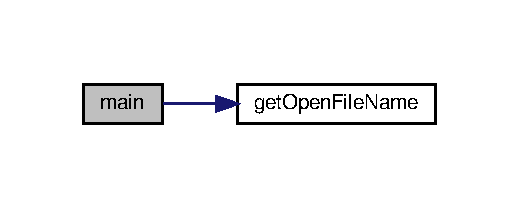
\includegraphics[width=249pt]{main_8cpp_ae66f6b31b5ad750f1fe042a706a4e3d4_cgraph}
\end{center}
\end{figure}

\hypertarget{system__target_8hpp}{}\section{Référence du fichier src/system\+\_\+target.hpp}
\label{system__target_8hpp}\index{src/system\+\_\+target.\+hpp@{src/system\+\_\+target.\+hpp}}
Ce graphe montre quels fichiers incluent directement ou indirectement ce fichier \+:\nopagebreak
\begin{figure}[H]
\begin{center}
\leavevmode
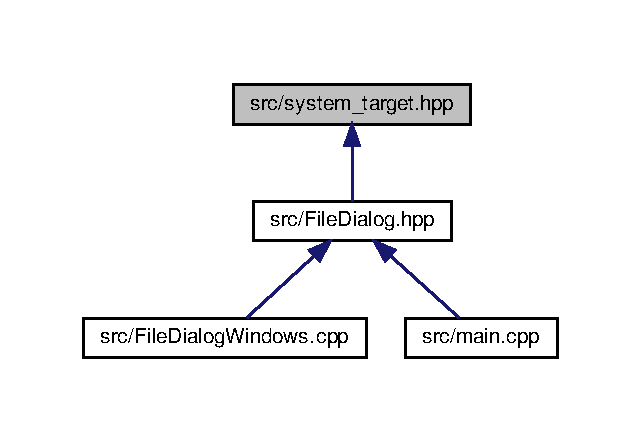
\includegraphics[width=199pt]{system__target_8hpp__dep__incl}
\end{center}
\end{figure}

\hypertarget{_tag_list_8hpp}{}\section{Référence du fichier src/\+Tag\+List.hpp}
\label{_tag_list_8hpp}\index{src/\+Tag\+List.\+hpp@{src/\+Tag\+List.\+hpp}}
{\ttfamily \#include $<$string$>$}\newline
{\ttfamily \#include $<$unordered\+\_\+set$>$}\newline
Graphe des dépendances par inclusion de Tag\+List.\+hpp\+:\nopagebreak
\begin{figure}[H]
\begin{center}
\leavevmode
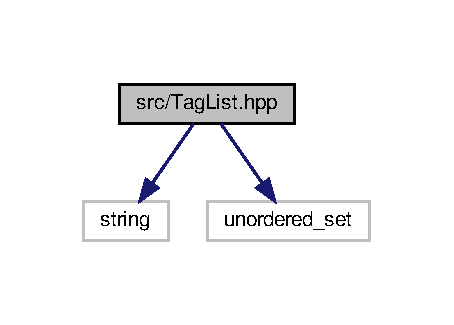
\includegraphics[width=218pt]{_tag_list_8hpp__incl}
\end{center}
\end{figure}
Ce graphe montre quels fichiers incluent directement ou indirectement ce fichier \+:\nopagebreak
\begin{figure}[H]
\begin{center}
\leavevmode
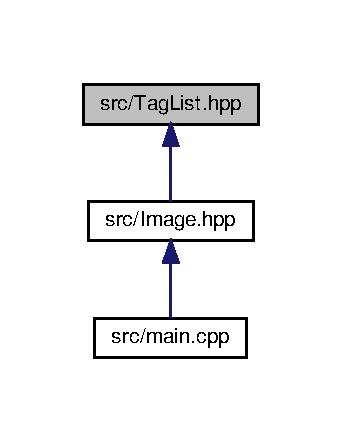
\includegraphics[width=164pt]{_tag_list_8hpp__dep__incl}
\end{center}
\end{figure}
\subsection*{Définitions de type}
\begin{DoxyCompactItemize}
\item 
using \hyperlink{_tag_list_8hpp_af037c70dc8c0318e30d3a5138776337e}{Tag} = std\+::string
\item 
using \hyperlink{_tag_list_8hpp_ac0222328791bb6c859b87ac65d5e9f65}{Tag\+List} = std\+::unordered\+\_\+set$<$ \hyperlink{_tag_list_8hpp_af037c70dc8c0318e30d3a5138776337e}{Tag} $>$
\end{DoxyCompactItemize}


\subsection{Documentation des définitions de type}
\mbox{\Hypertarget{_tag_list_8hpp_af037c70dc8c0318e30d3a5138776337e}\label{_tag_list_8hpp_af037c70dc8c0318e30d3a5138776337e}} 
\index{Tag\+List.\+hpp@{Tag\+List.\+hpp}!Tag@{Tag}}
\index{Tag@{Tag}!Tag\+List.\+hpp@{Tag\+List.\+hpp}}
\subsubsection{\texorpdfstring{Tag}{Tag}}
{\footnotesize\ttfamily using \hyperlink{_tag_list_8hpp_af037c70dc8c0318e30d3a5138776337e}{Tag} =  std\+::string}

\mbox{\Hypertarget{_tag_list_8hpp_ac0222328791bb6c859b87ac65d5e9f65}\label{_tag_list_8hpp_ac0222328791bb6c859b87ac65d5e9f65}} 
\index{Tag\+List.\+hpp@{Tag\+List.\+hpp}!Tag\+List@{Tag\+List}}
\index{Tag\+List@{Tag\+List}!Tag\+List.\+hpp@{Tag\+List.\+hpp}}
\subsubsection{\texorpdfstring{Tag\+List}{TagList}}
{\footnotesize\ttfamily using \hyperlink{_tag_list_8hpp_ac0222328791bb6c859b87ac65d5e9f65}{Tag\+List} =  std\+::unordered\+\_\+set$<$\hyperlink{_tag_list_8hpp_af037c70dc8c0318e30d3a5138776337e}{Tag}$>$}


\hypertarget{_window_8hpp}{}\section{Référence du fichier src/\+Window.hpp}
\label{_window_8hpp}\index{src/\+Window.\+hpp@{src/\+Window.\+hpp}}

%--- End generated contents ---

% Index
\backmatter
\newpage
\phantomsection
\clearemptydoublepage
\addcontentsline{toc}{chapter}{Index}
\printindex

\end{document}
